\section{Jet Energy Resolution Calculation}
\label{app:jer}
Jet energy resolution is calculted in the following ways:
\begin{itemize}
\item We category the jet in six $p_{T}$ bins: [30, 50, 70, 100, 200, 300, 500] and five $|\eta|$ bins: [0.0, 0.5, 1.1, 1.7, 2.3, 5.0]
\item We match the Reco jet with Gen jet and then fit (Reojet $p_{T}$ - Genjet $p_{T}$)/Genjet $p_{T}$ distribution to get jet $\sigma_{MC}$
\end{itemize}

All the JER distribution and fit results show on the Figs.~\ref{fig:jer_eta_1_pt_1} to Figs.~\ref{fig:jer_eta_5_pt_5}

\begin{figure}[ht]{\centering
\unitlength=0.33\linewidth
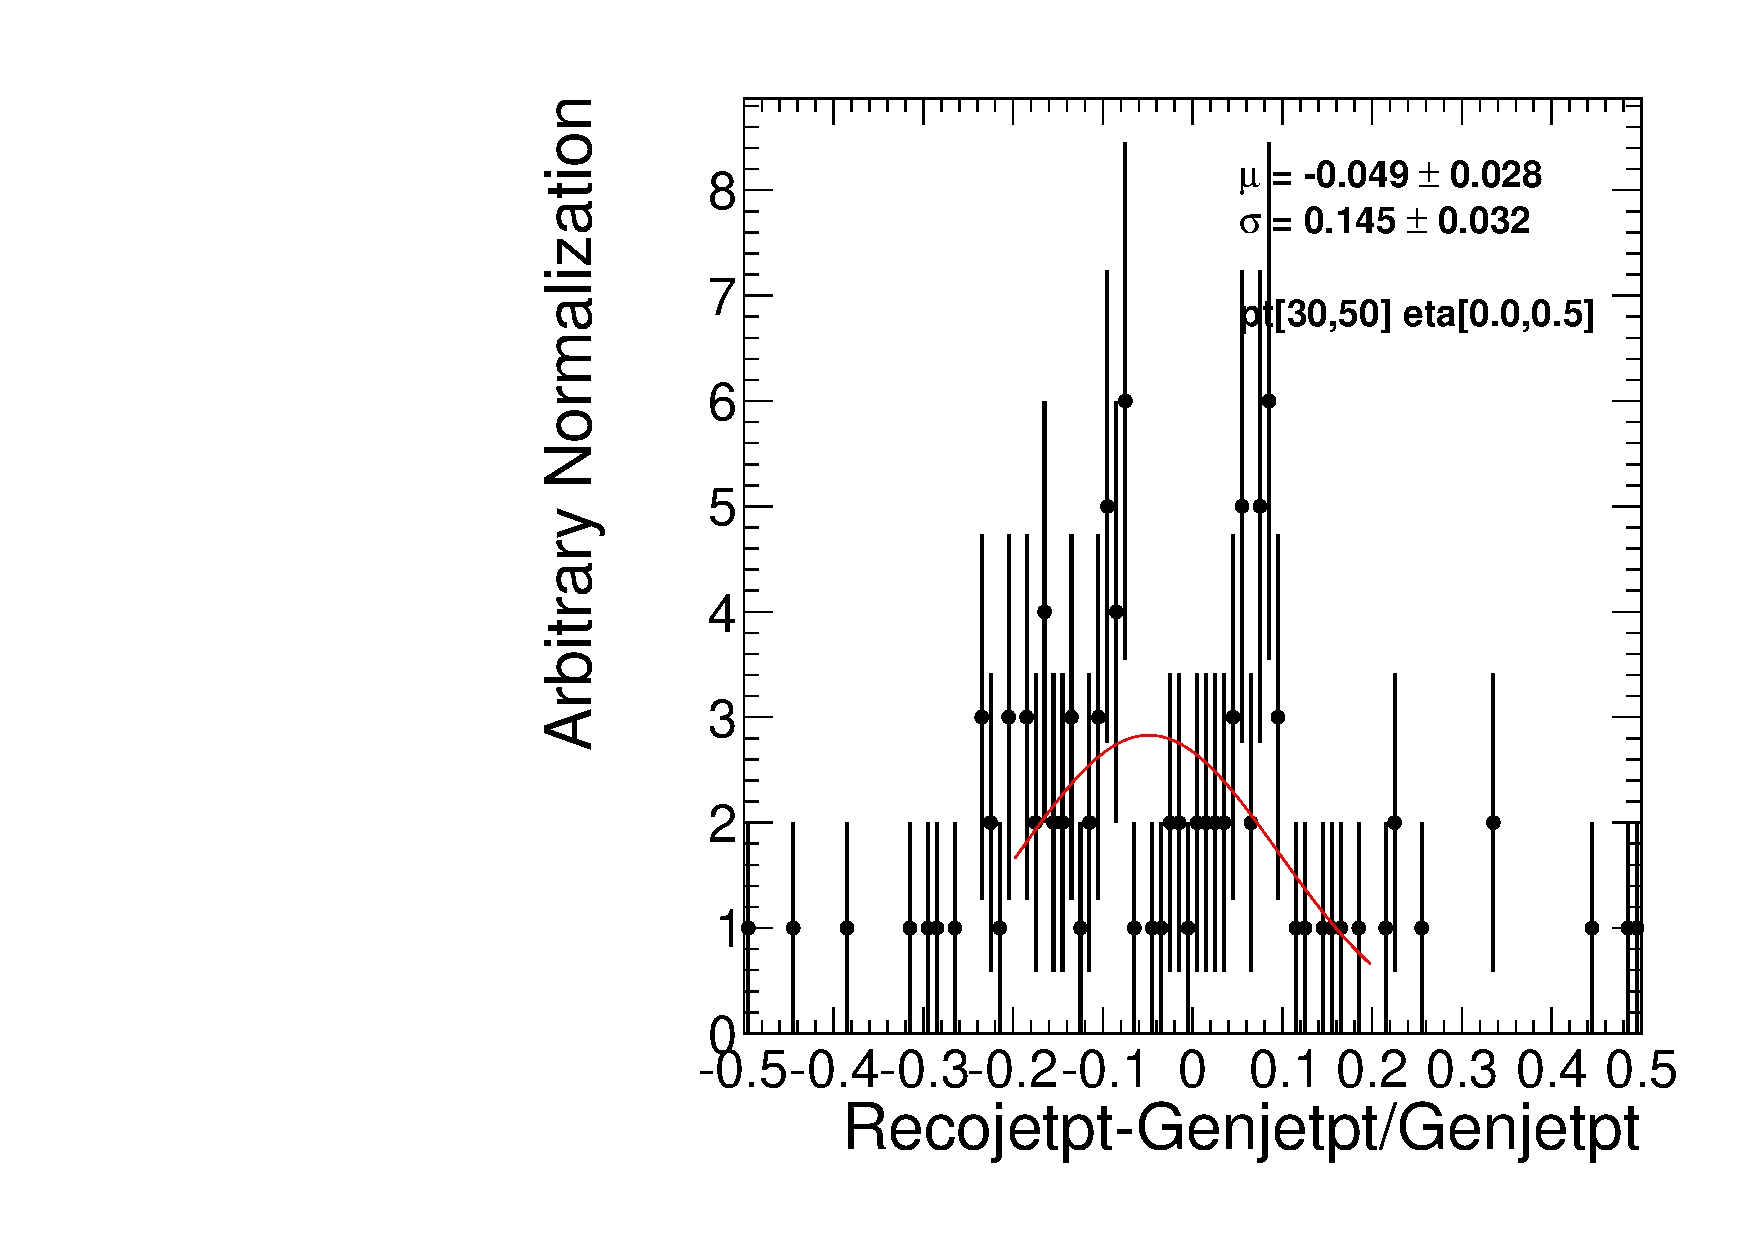
\includegraphics[width=0.45\textwidth]{figs/jer/mu_Recojetpt_Genjetpt_Genjetpt_0_0_0_5_30_50_tagjetresolution_jetresolution.pdf}
\put(-0.80,0.0){(a)}
\unitlength=0.33\linewidth
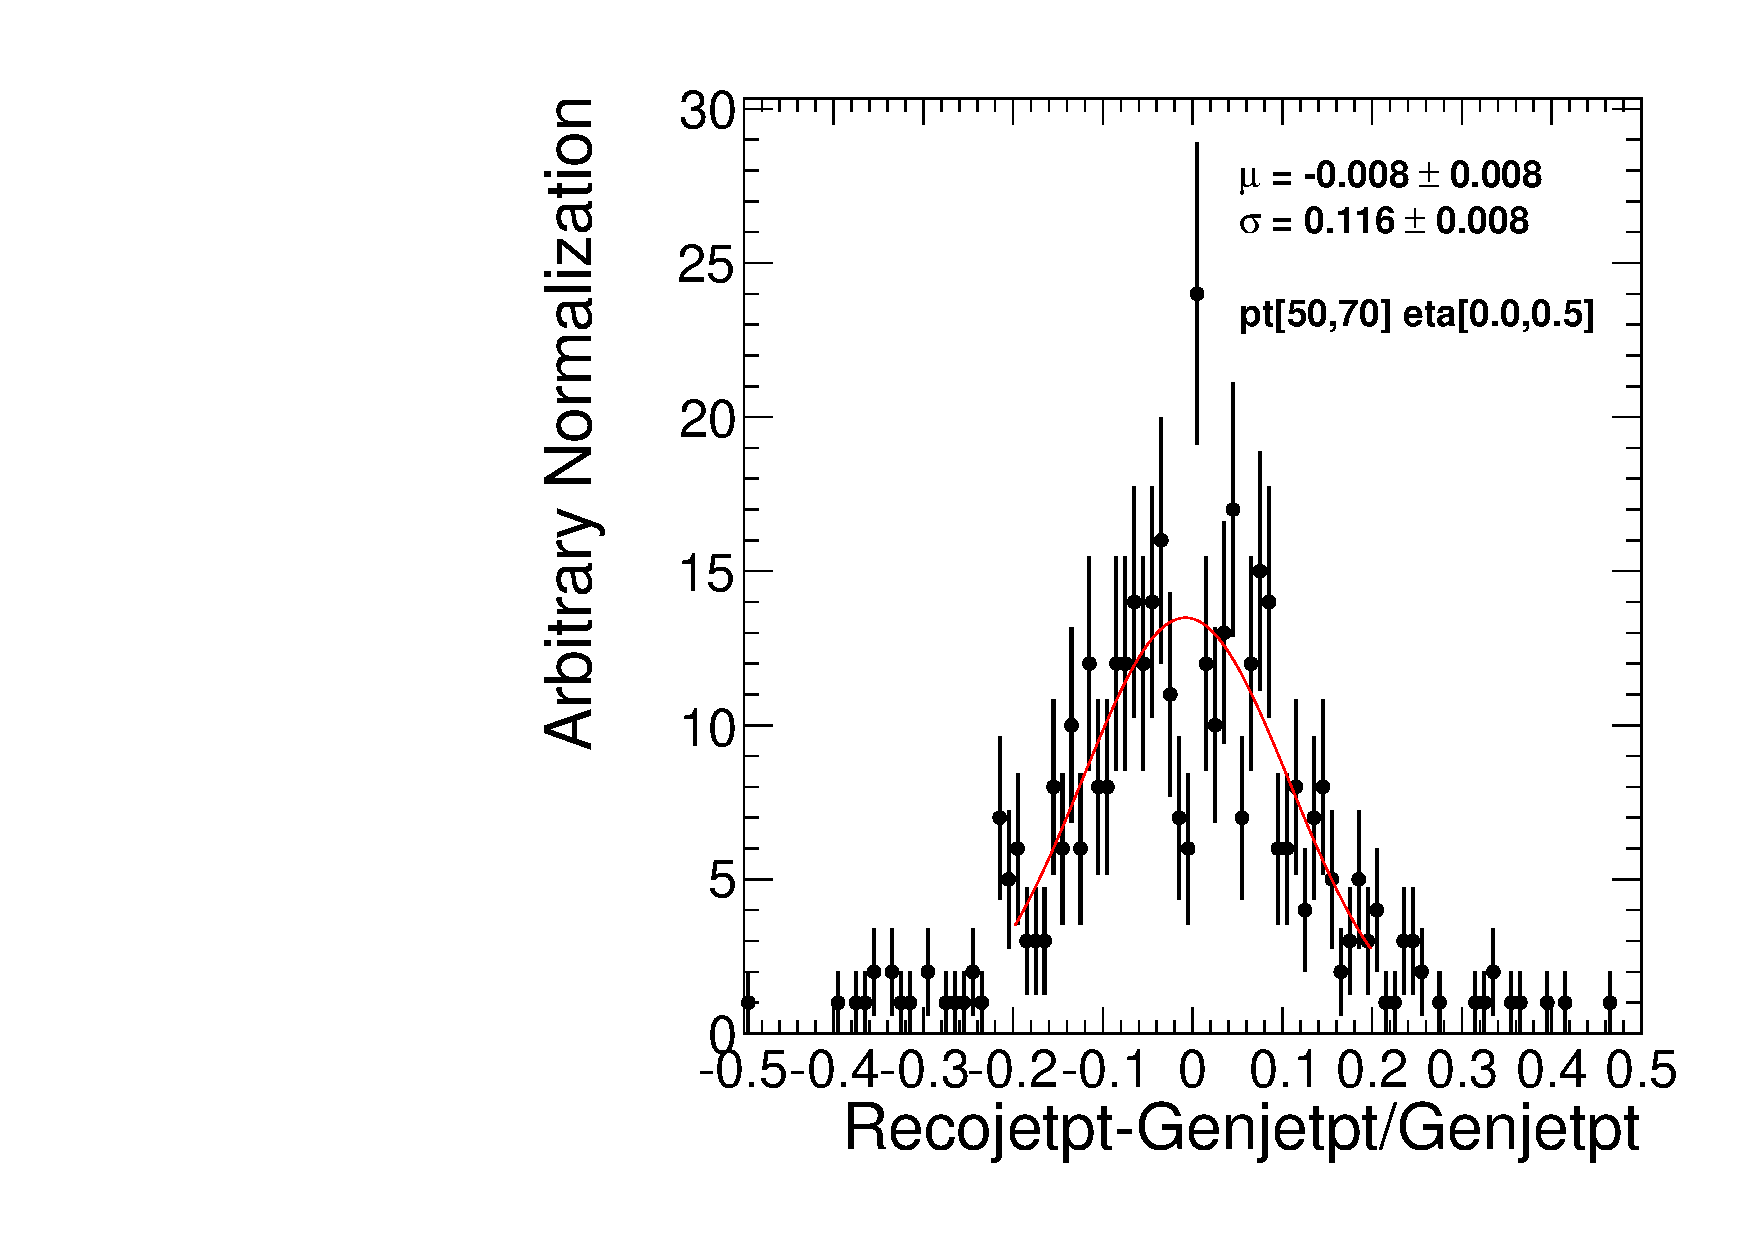
\includegraphics[width=0.45\textwidth]{figs/jer/mu_Recojetpt_Genjetpt_Genjetpt_0_0_0_5_50_70_tagjetresolution_jetresolution.pdf}
\put(-0.80,0.0){(b)} \\  
\unitlength=0.33\linewidth
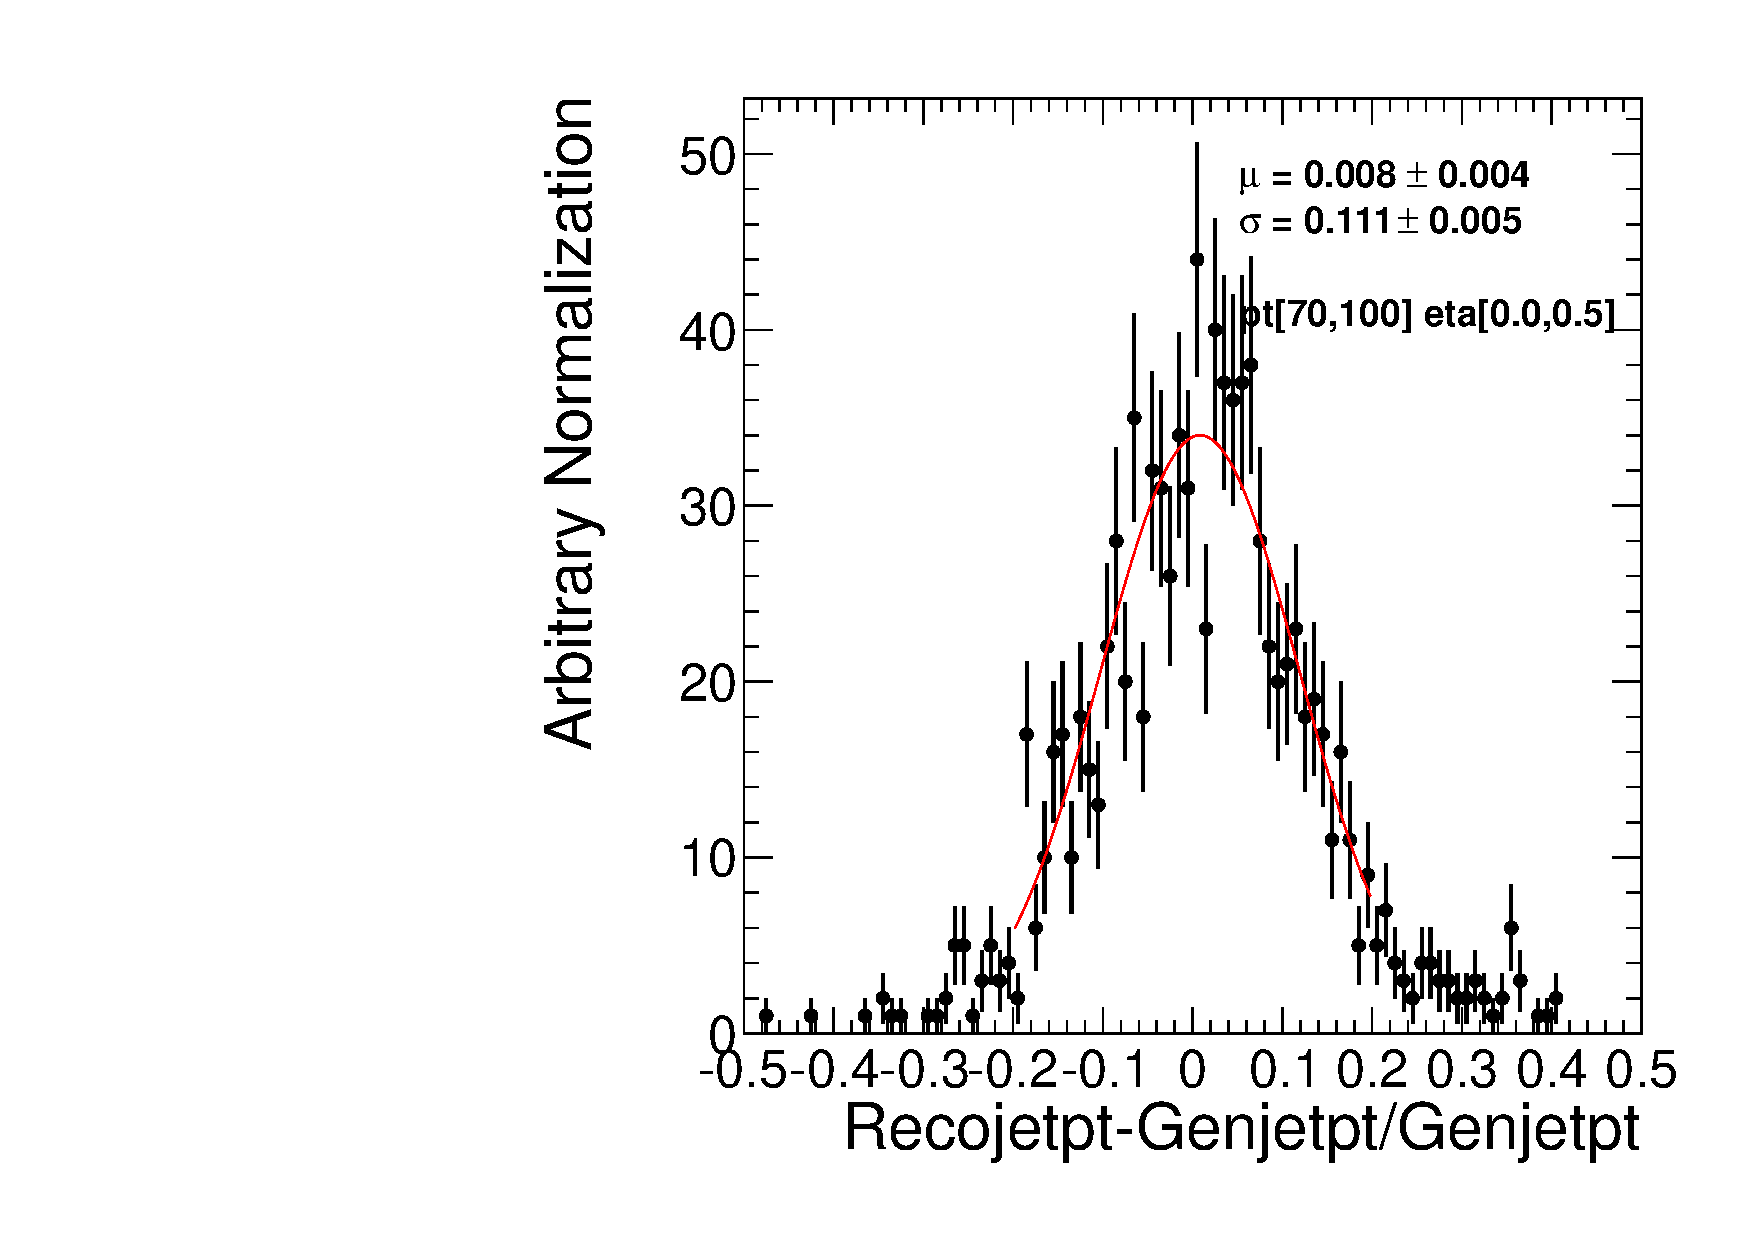
\includegraphics[width=0.45\textwidth]{figs/jer/mu_Recojetpt_Genjetpt_Genjetpt_0_0_0_5_70_100_tagjetresolution_jetresolution.pdf}
\put(-0.80,0.0){(c)}
\unitlength=0.33\linewidth
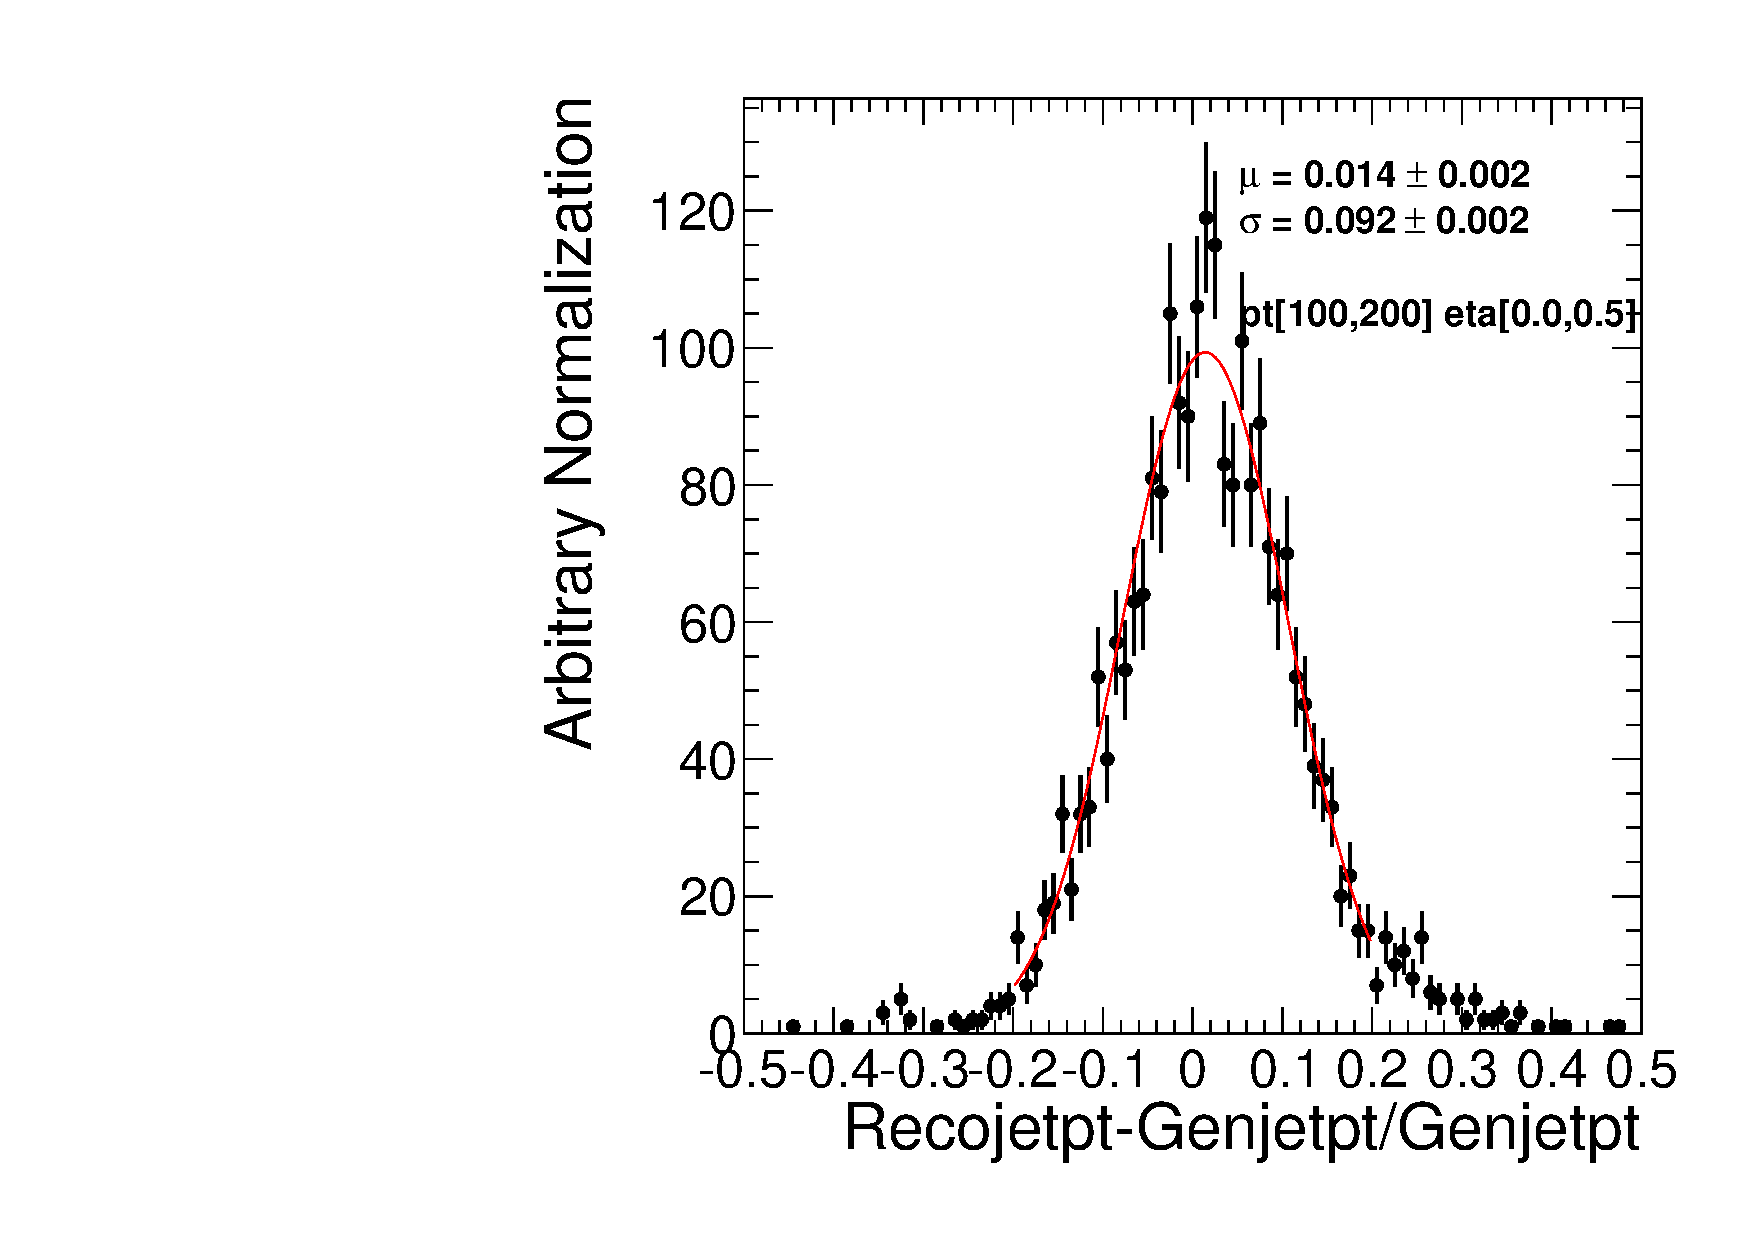
\includegraphics[width=0.45\textwidth]{figs/jer/mu_Recojetpt_Genjetpt_Genjetpt_0_0_0_5_100_200_tagjetresolution_jetresolution.pdf}
\put(-0.80,0.0){(d)}\\ 
\unitlength=0.33\linewidth
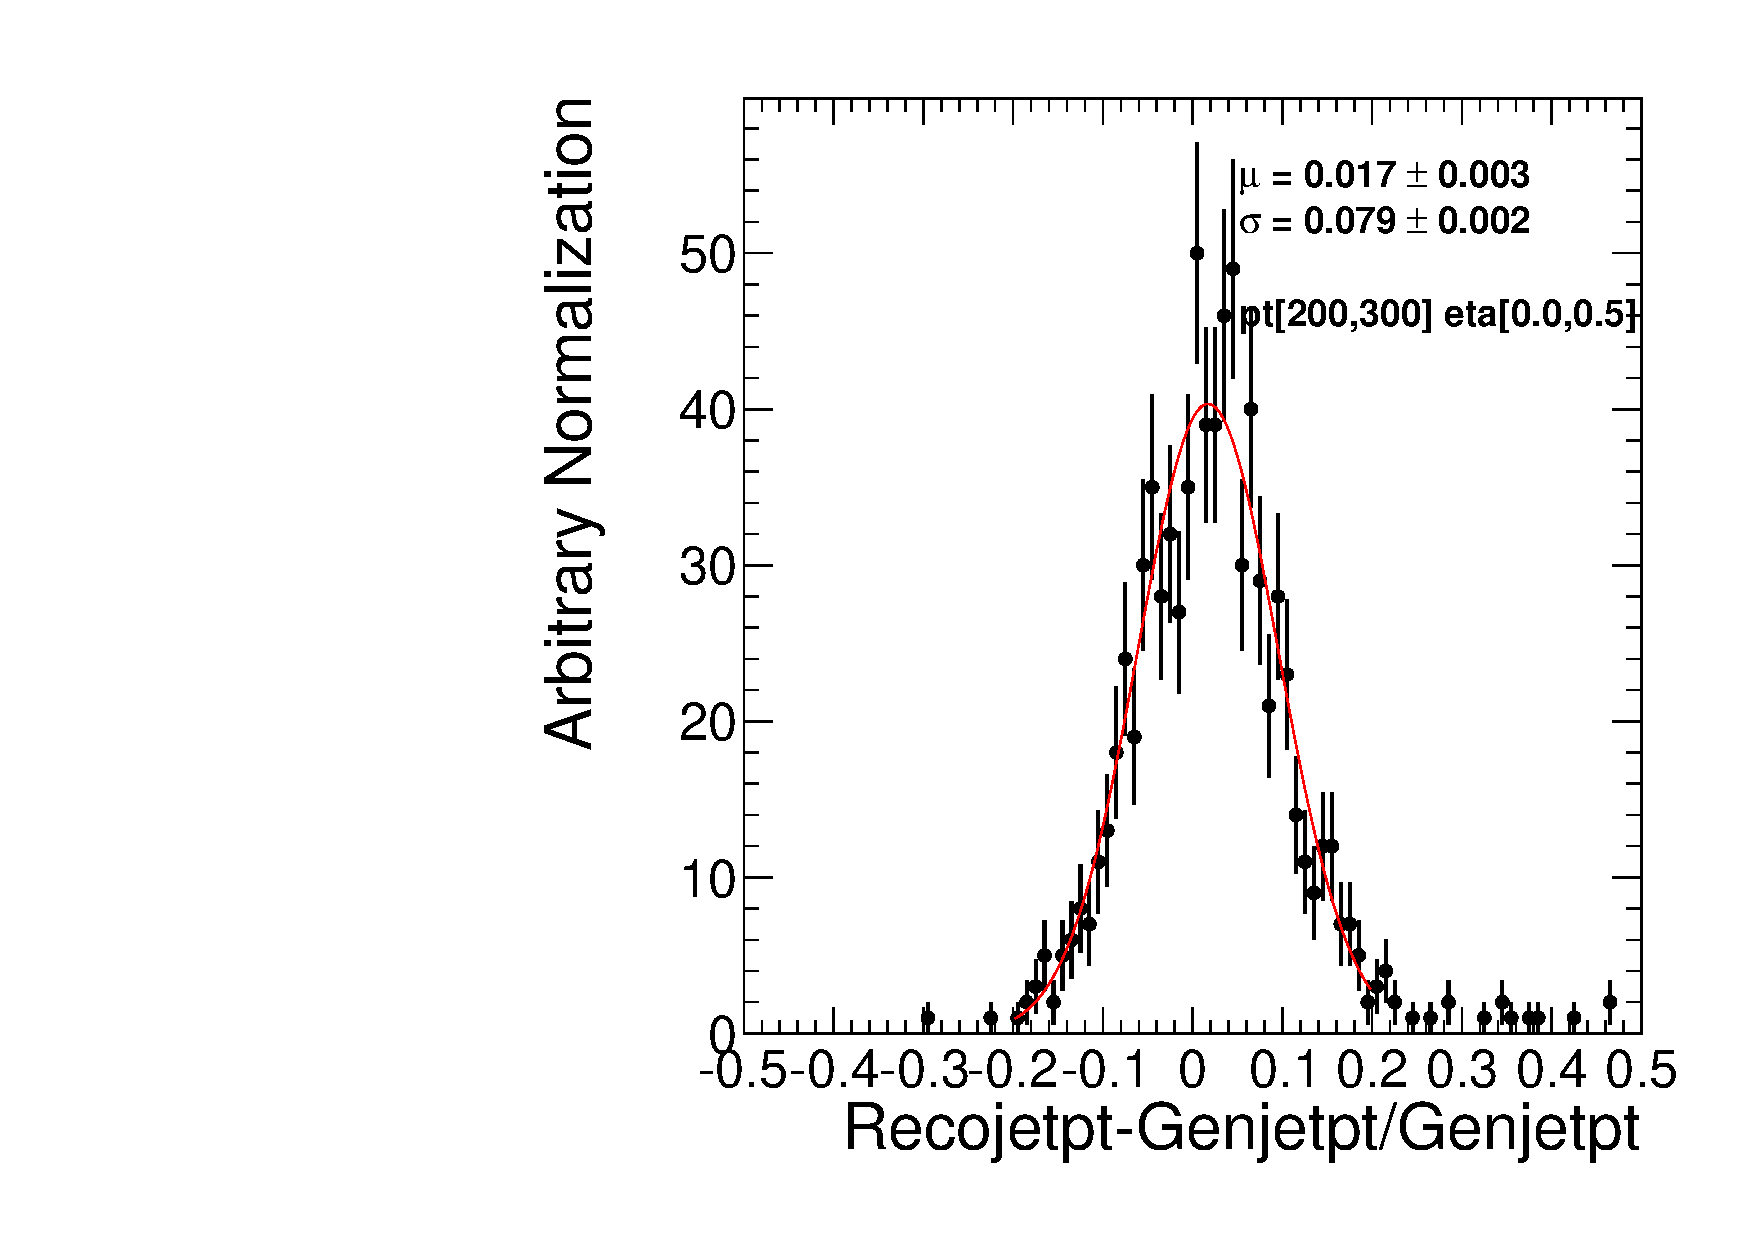
\includegraphics[width=0.45\textwidth]{figs/jer/mu_Recojetpt_Genjetpt_Genjetpt_0_0_0_5_200_300_tagjetresolution_jetresolution.pdf}
\put(-0.80,0.0){(e)} 
\unitlength=0.33\linewidth
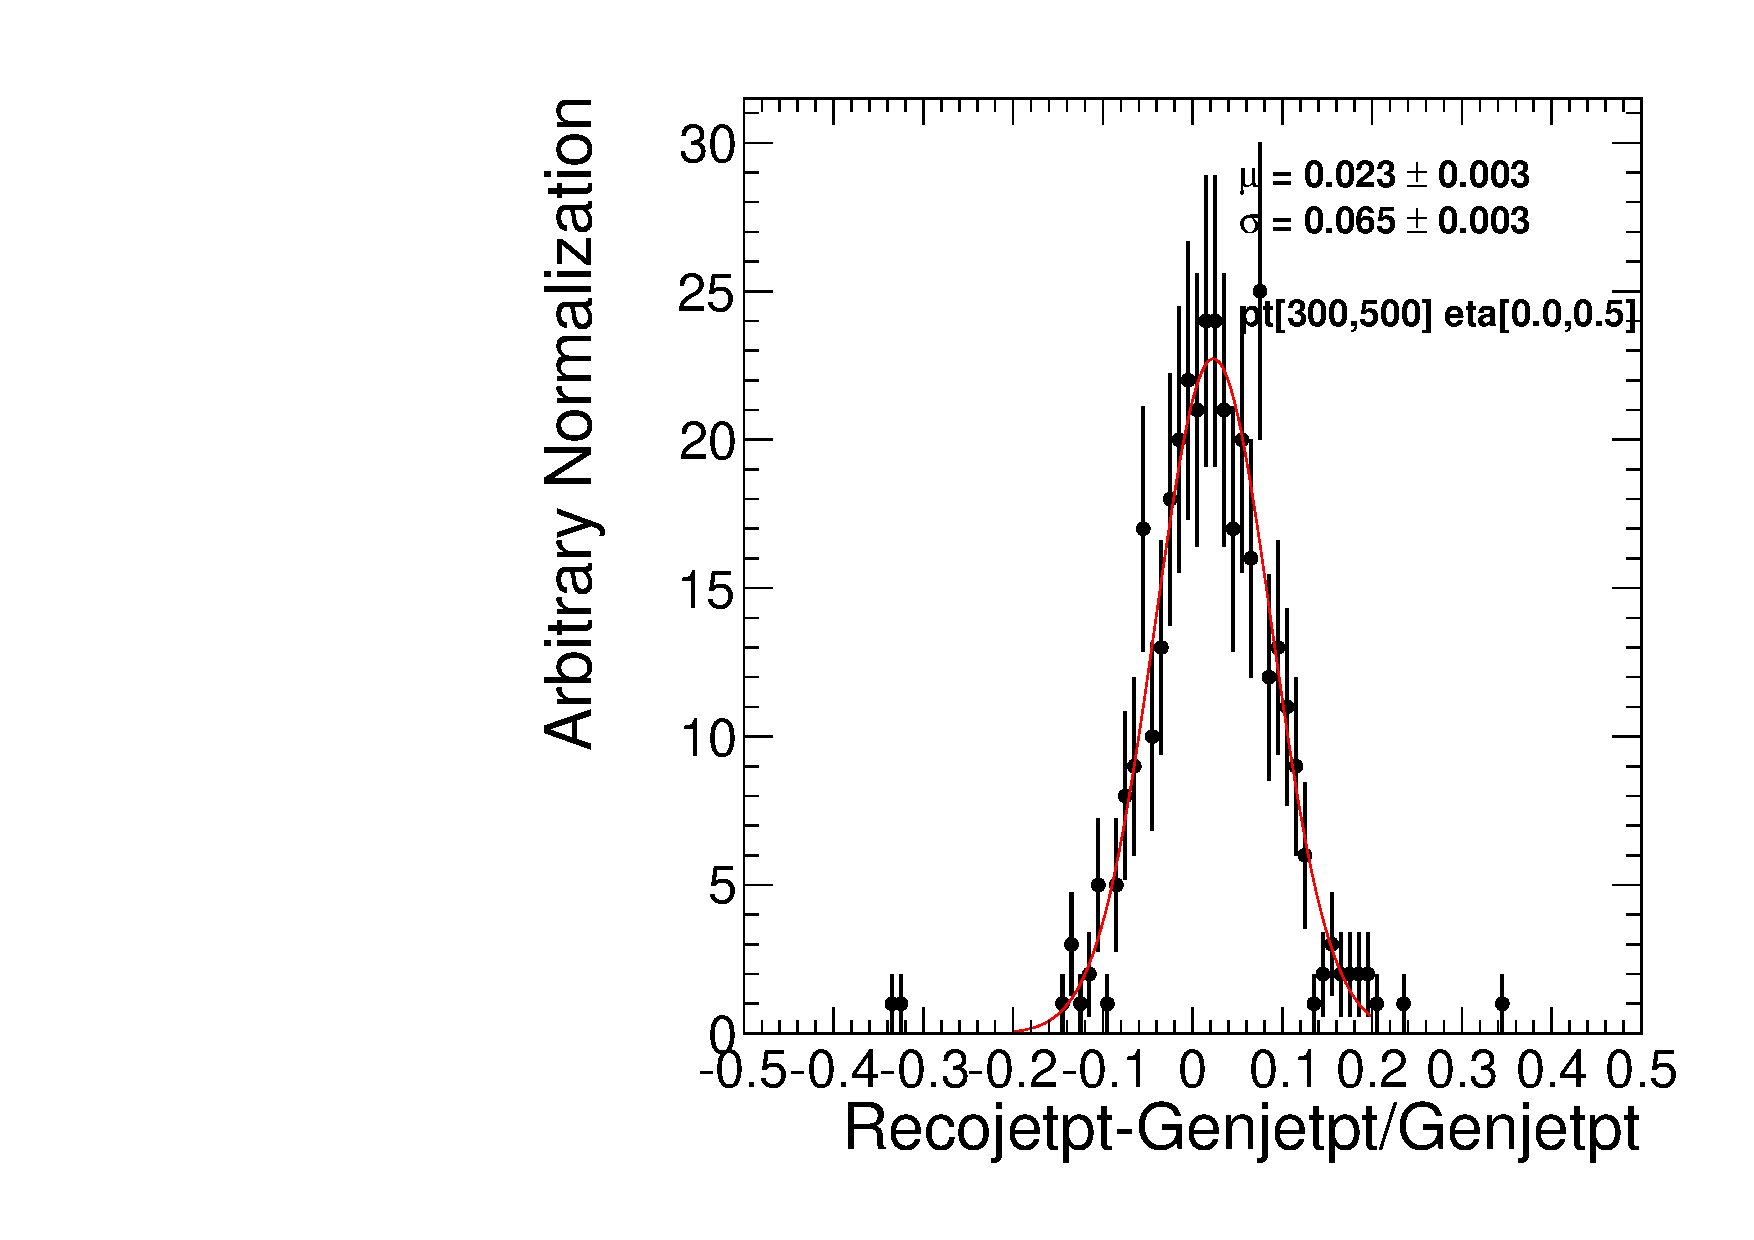
\includegraphics[width=0.45\textwidth]{figs/jer/mu_Recojetpt_Genjetpt_Genjetpt_0_0_0_5_300_500_tagjetresolution_jetresolution.pdf}
\put(-0.80,0.0){(f)} 
\caption{Fit result in jet $\eta$ bin: [0.0, 0.5] for six $p_{T}$[GeV/c] bins: 
         (a) [30, 50], (b) [50, 70], (b) [70, 100], (d) [100, 200], (e) [200, 300], (f) [300, 500].}
\label{fig:jer_eta_1_pt_1}}
\end{figure}

\begin{figure}[ht]{\centering
\unitlength=0.33\linewidth
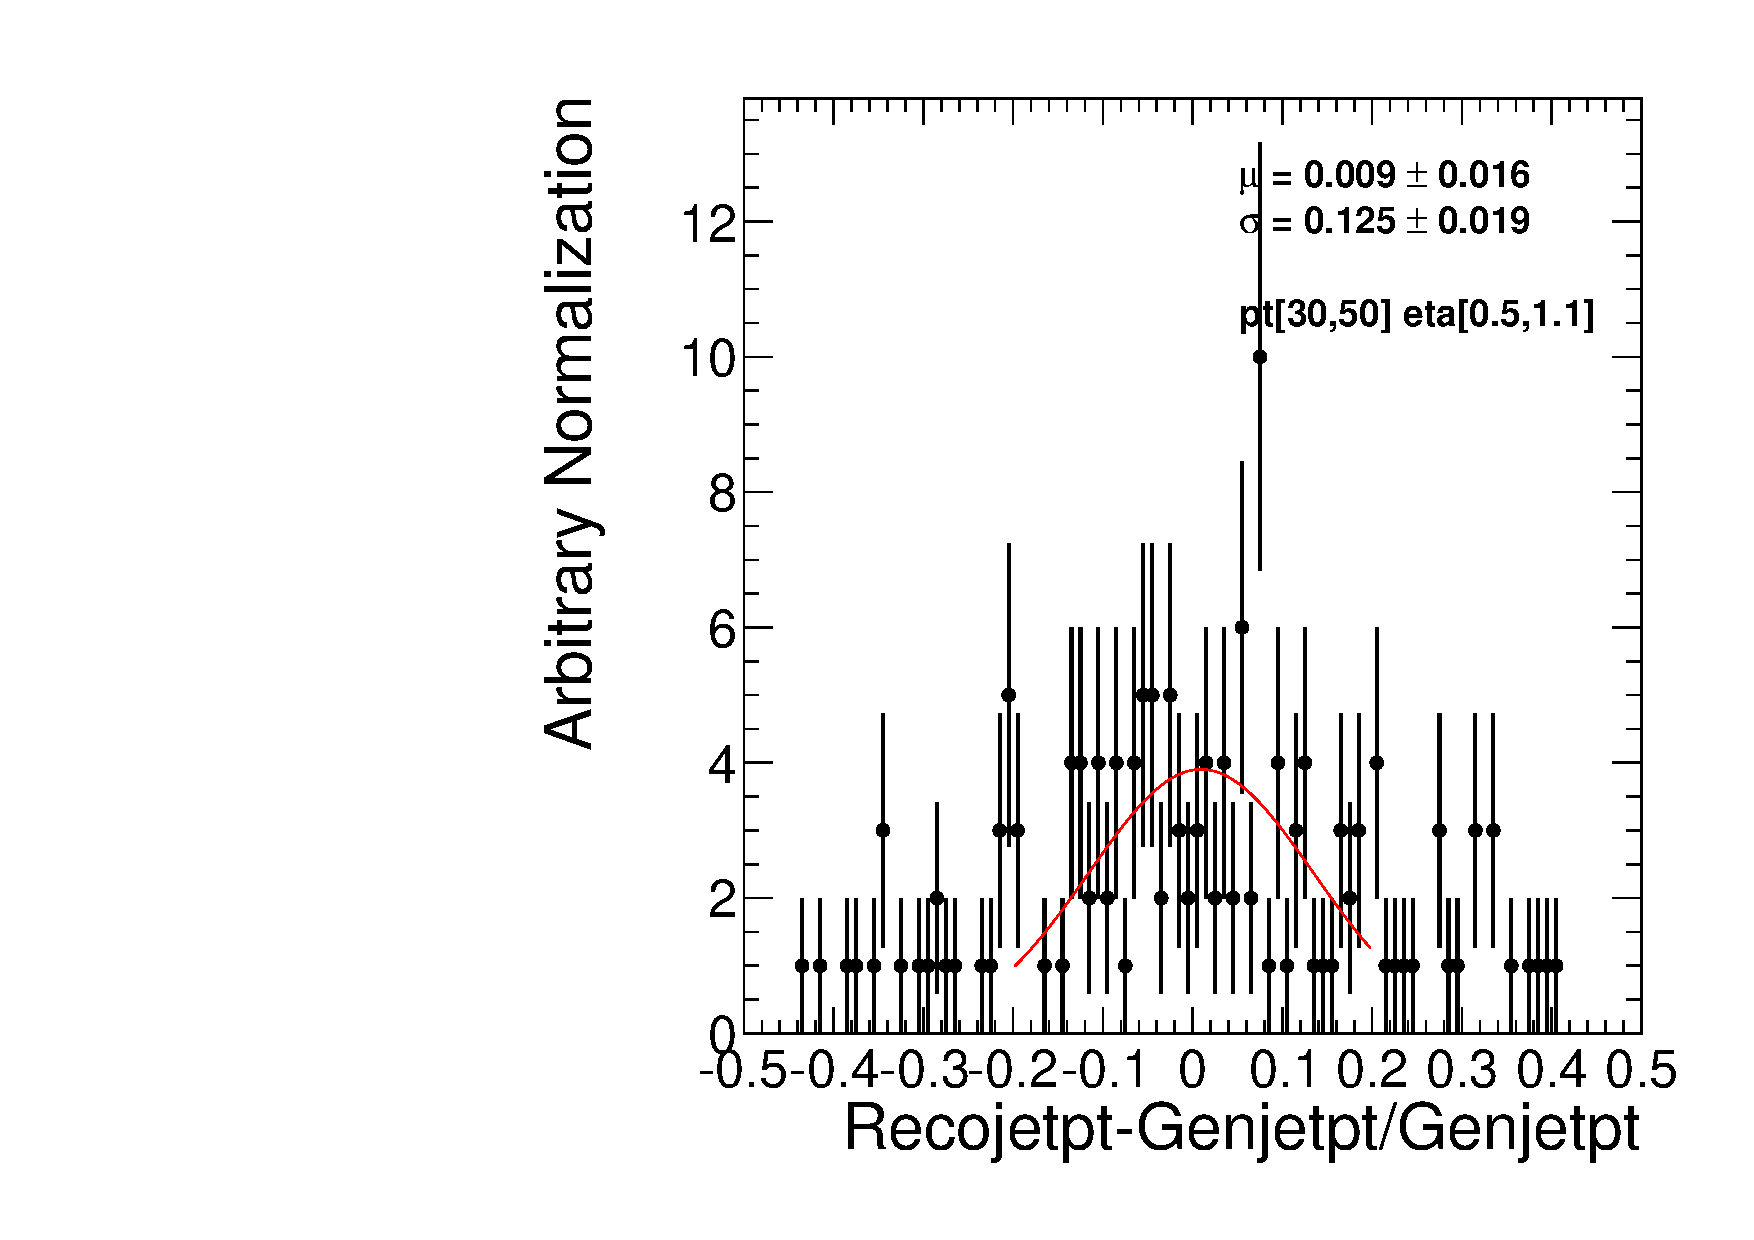
\includegraphics[width=0.45\textwidth]{figs/jer/mu_Recojetpt_Genjetpt_Genjetpt_0_5_1_1_30_50_tagjetresolution_jetresolution.pdf}
\put(-0.80,0.0){(a)}
\unitlength=0.33\linewidth
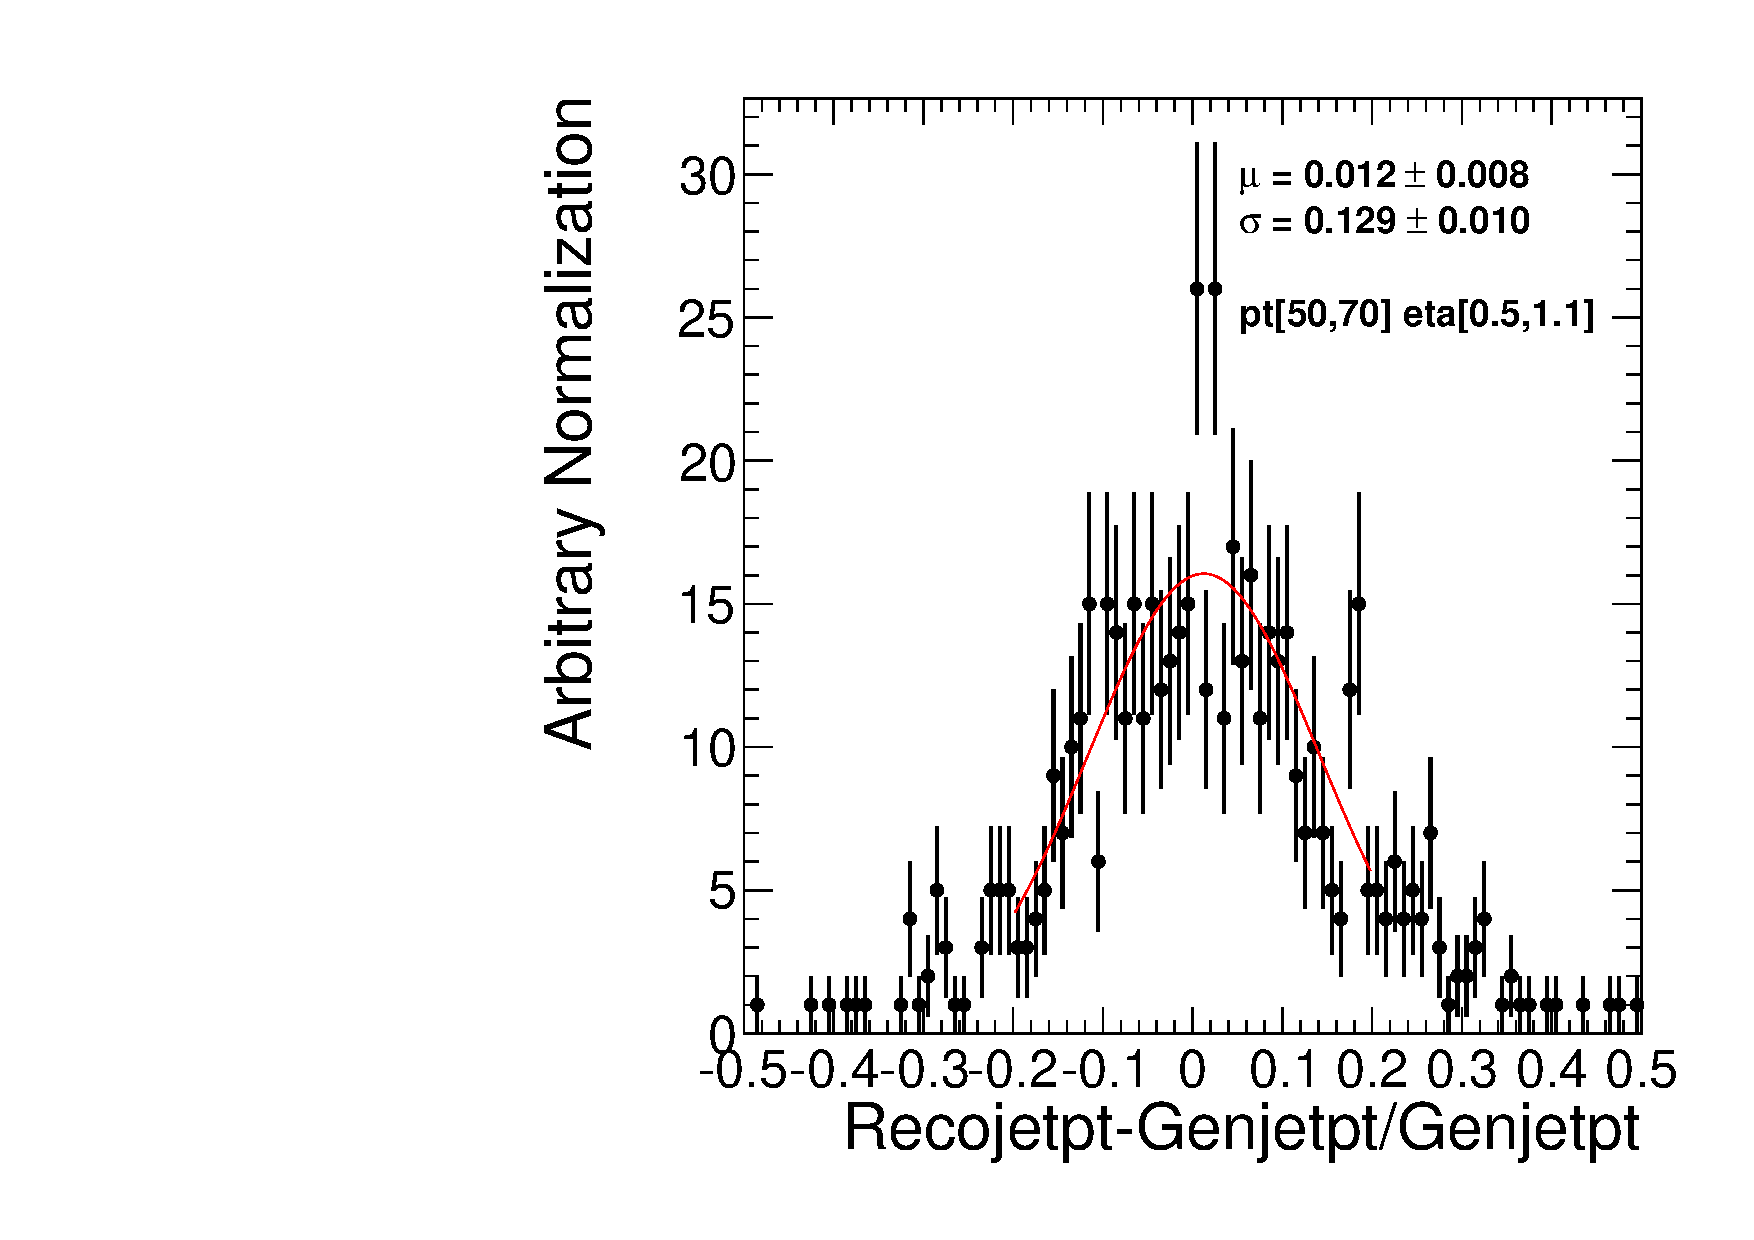
\includegraphics[width=0.45\textwidth]{figs/jer/mu_Recojetpt_Genjetpt_Genjetpt_0_5_1_1_50_70_tagjetresolution_jetresolution.pdf}
\put(-0.80,0.0){(b)} \\  
\unitlength=0.33\linewidth
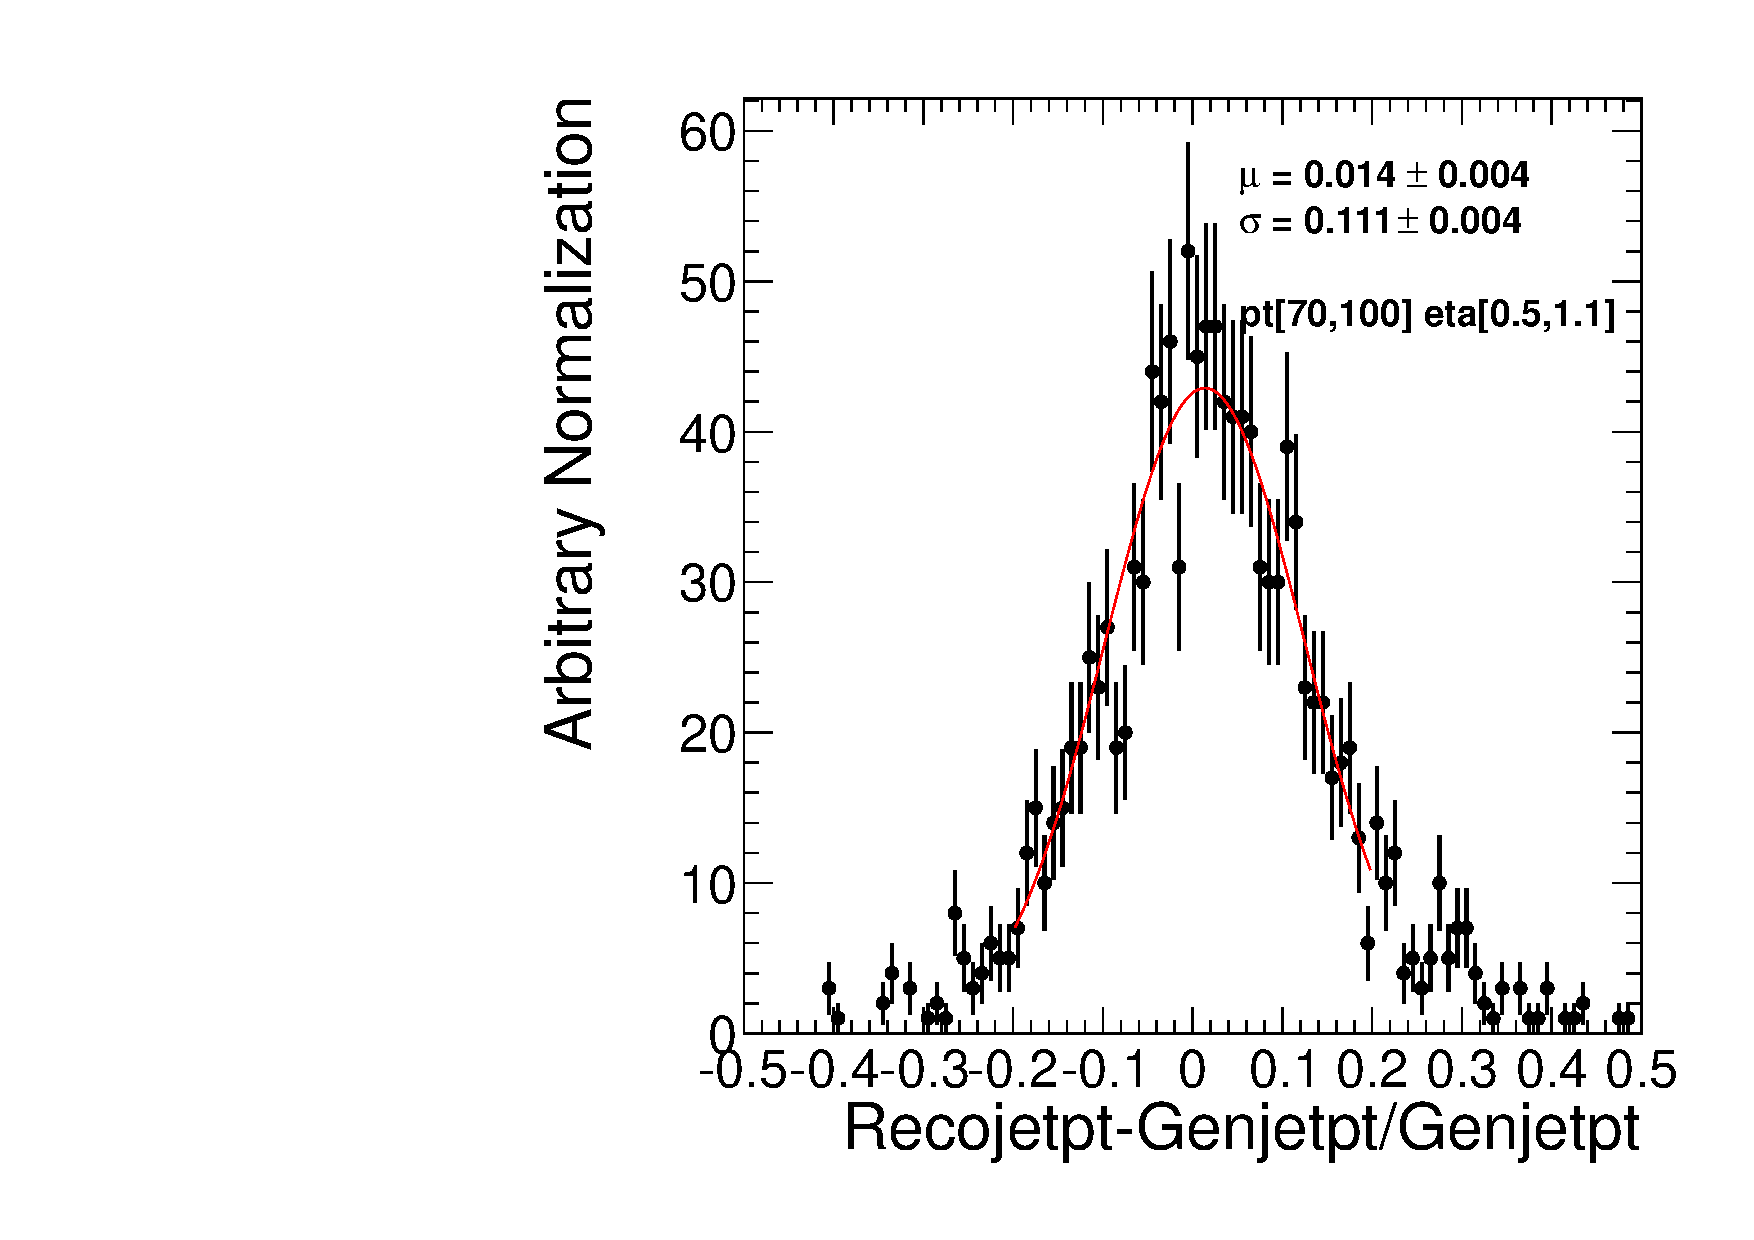
\includegraphics[width=0.45\textwidth]{figs/jer/mu_Recojetpt_Genjetpt_Genjetpt_0_5_1_1_70_100_tagjetresolution_jetresolution.pdf}
\put(-0.80,0.0){(c)}
\unitlength=0.33\linewidth
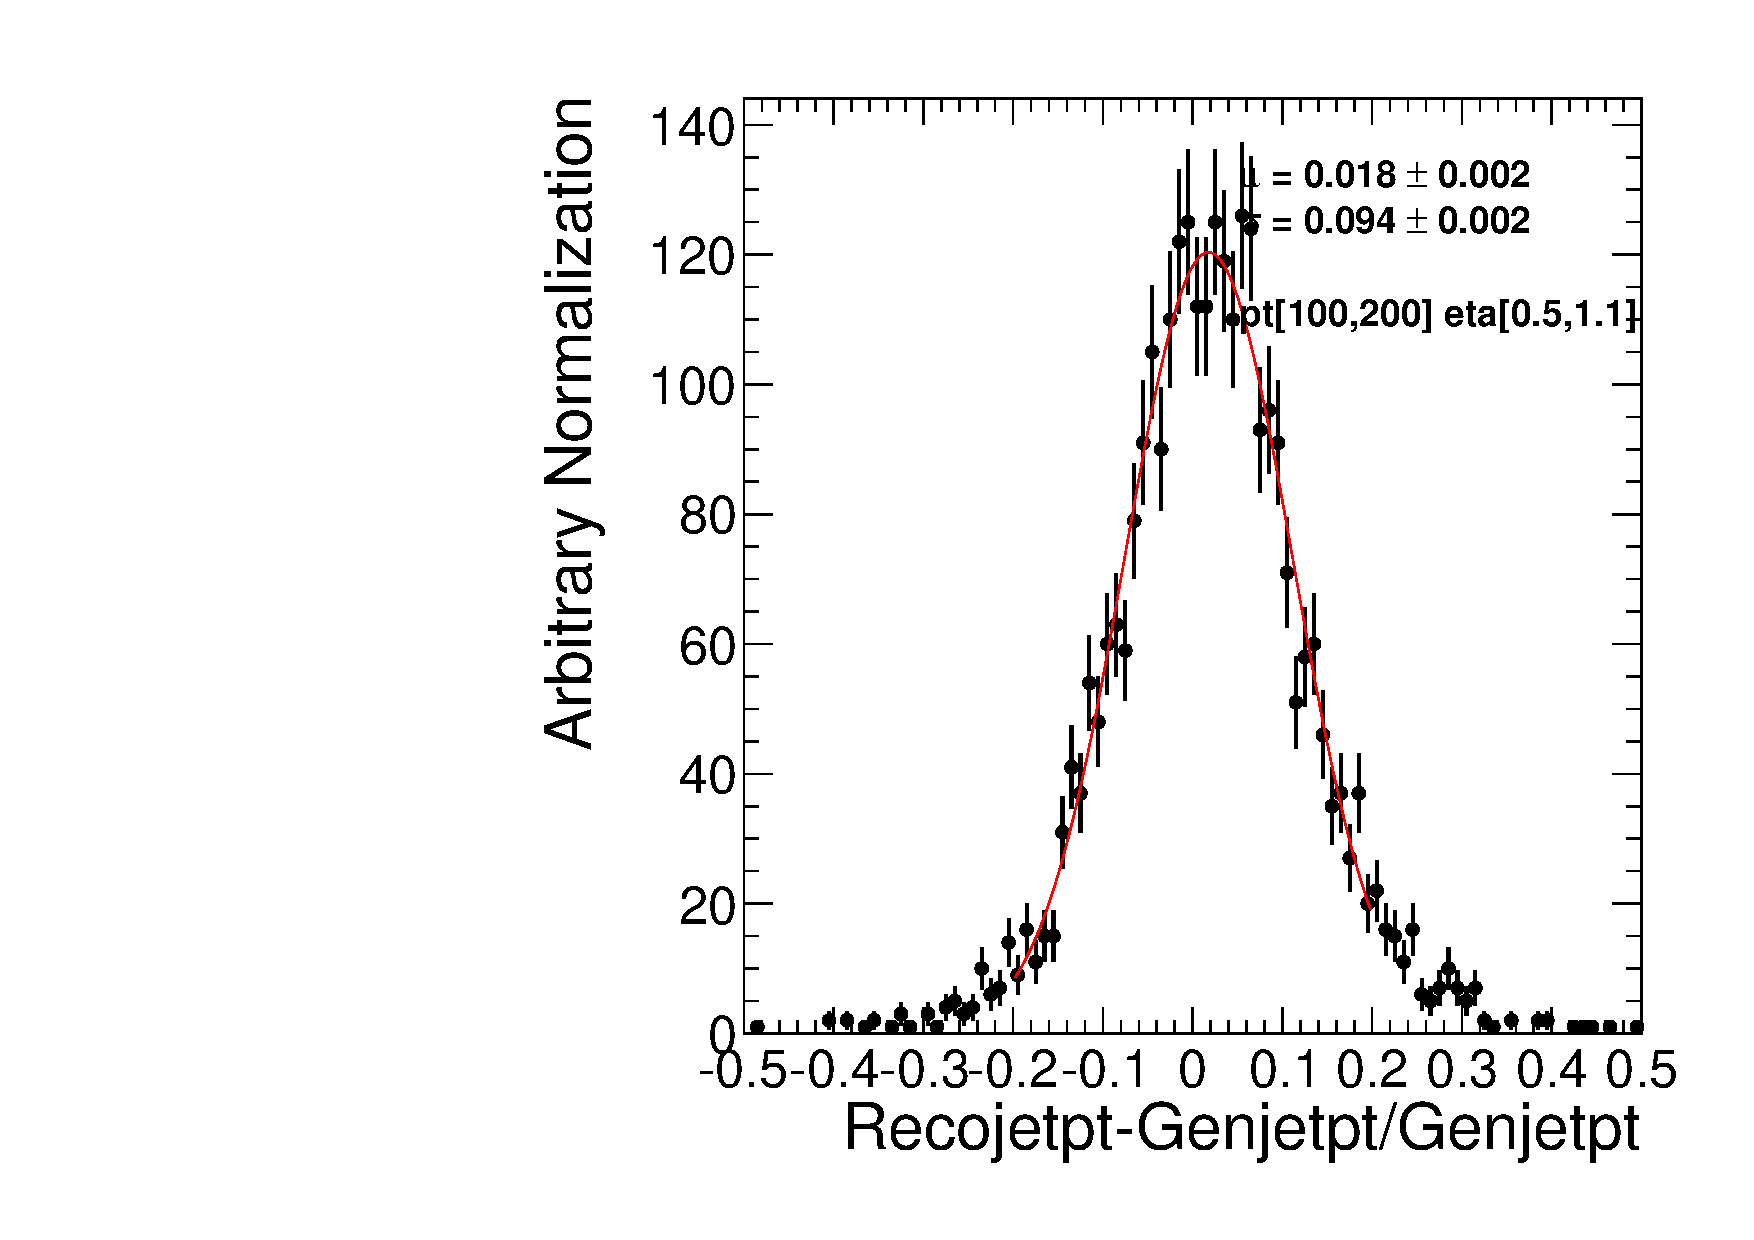
\includegraphics[width=0.45\textwidth]{figs/jer/mu_Recojetpt_Genjetpt_Genjetpt_0_5_1_1_100_200_tagjetresolution_jetresolution.pdf}
\put(-0.80,0.0){(d)}\\ 
\unitlength=0.33\linewidth
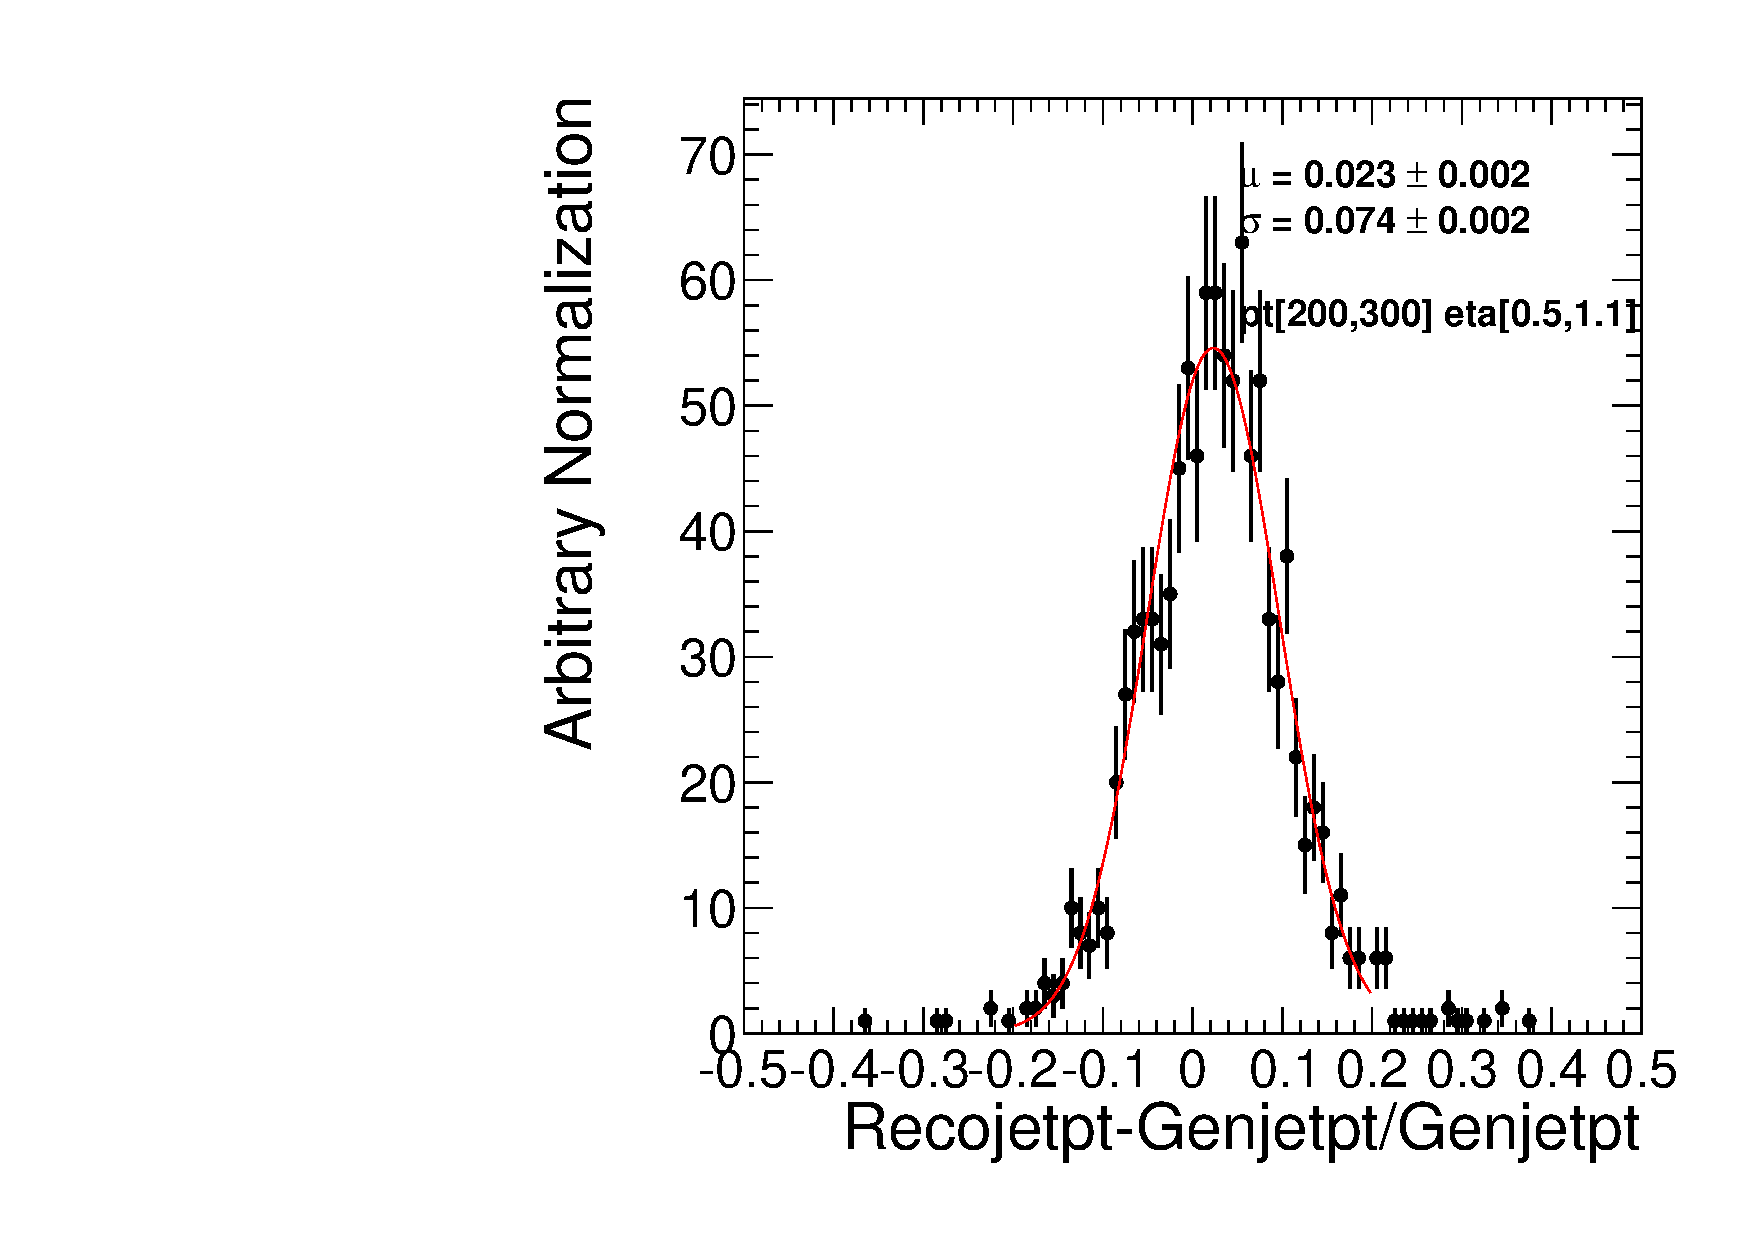
\includegraphics[width=0.45\textwidth]{figs/jer/mu_Recojetpt_Genjetpt_Genjetpt_0_5_1_1_200_300_tagjetresolution_jetresolution.pdf}
\put(-0.80,0.0){(e)} 
\unitlength=0.33\linewidth
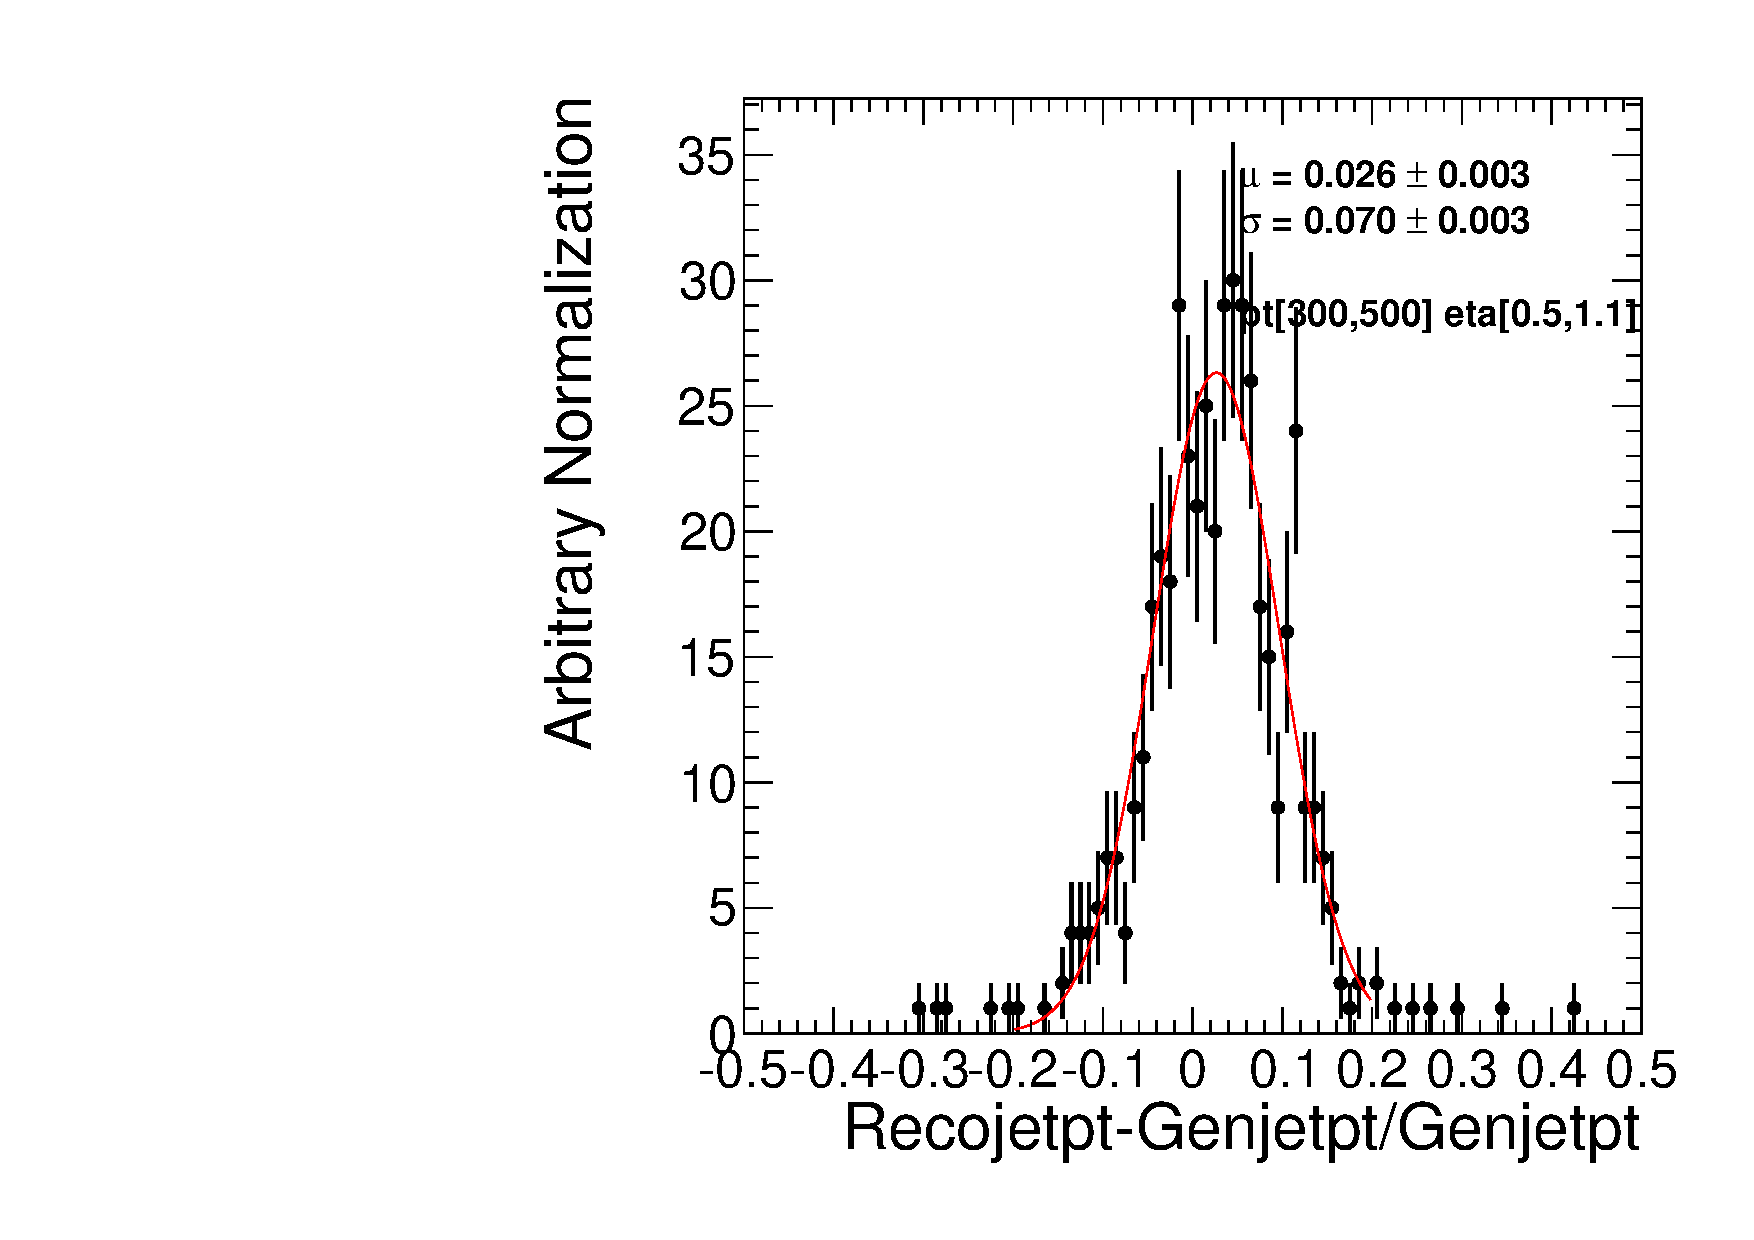
\includegraphics[width=0.45\textwidth]{figs/jer/mu_Recojetpt_Genjetpt_Genjetpt_0_5_1_1_300_500_tagjetresolution_jetresolution.pdf}
\put(-0.80,0.0){(f)} 
\caption{Fit result in jet $\eta$ bin: [0.5, 1.1] for six $p_{T}$[GeV/c] bins: 
         (a) [30, 50], (b) [50, 70], (b) [70, 100], (d) [100, 200], (e) [200, 300], (f) [300, 500].}
\label{fig:jer_eta_2_pt_2}}
\end{figure}

\begin{figure}[ht]{\centering
\unitlength=0.33\linewidth
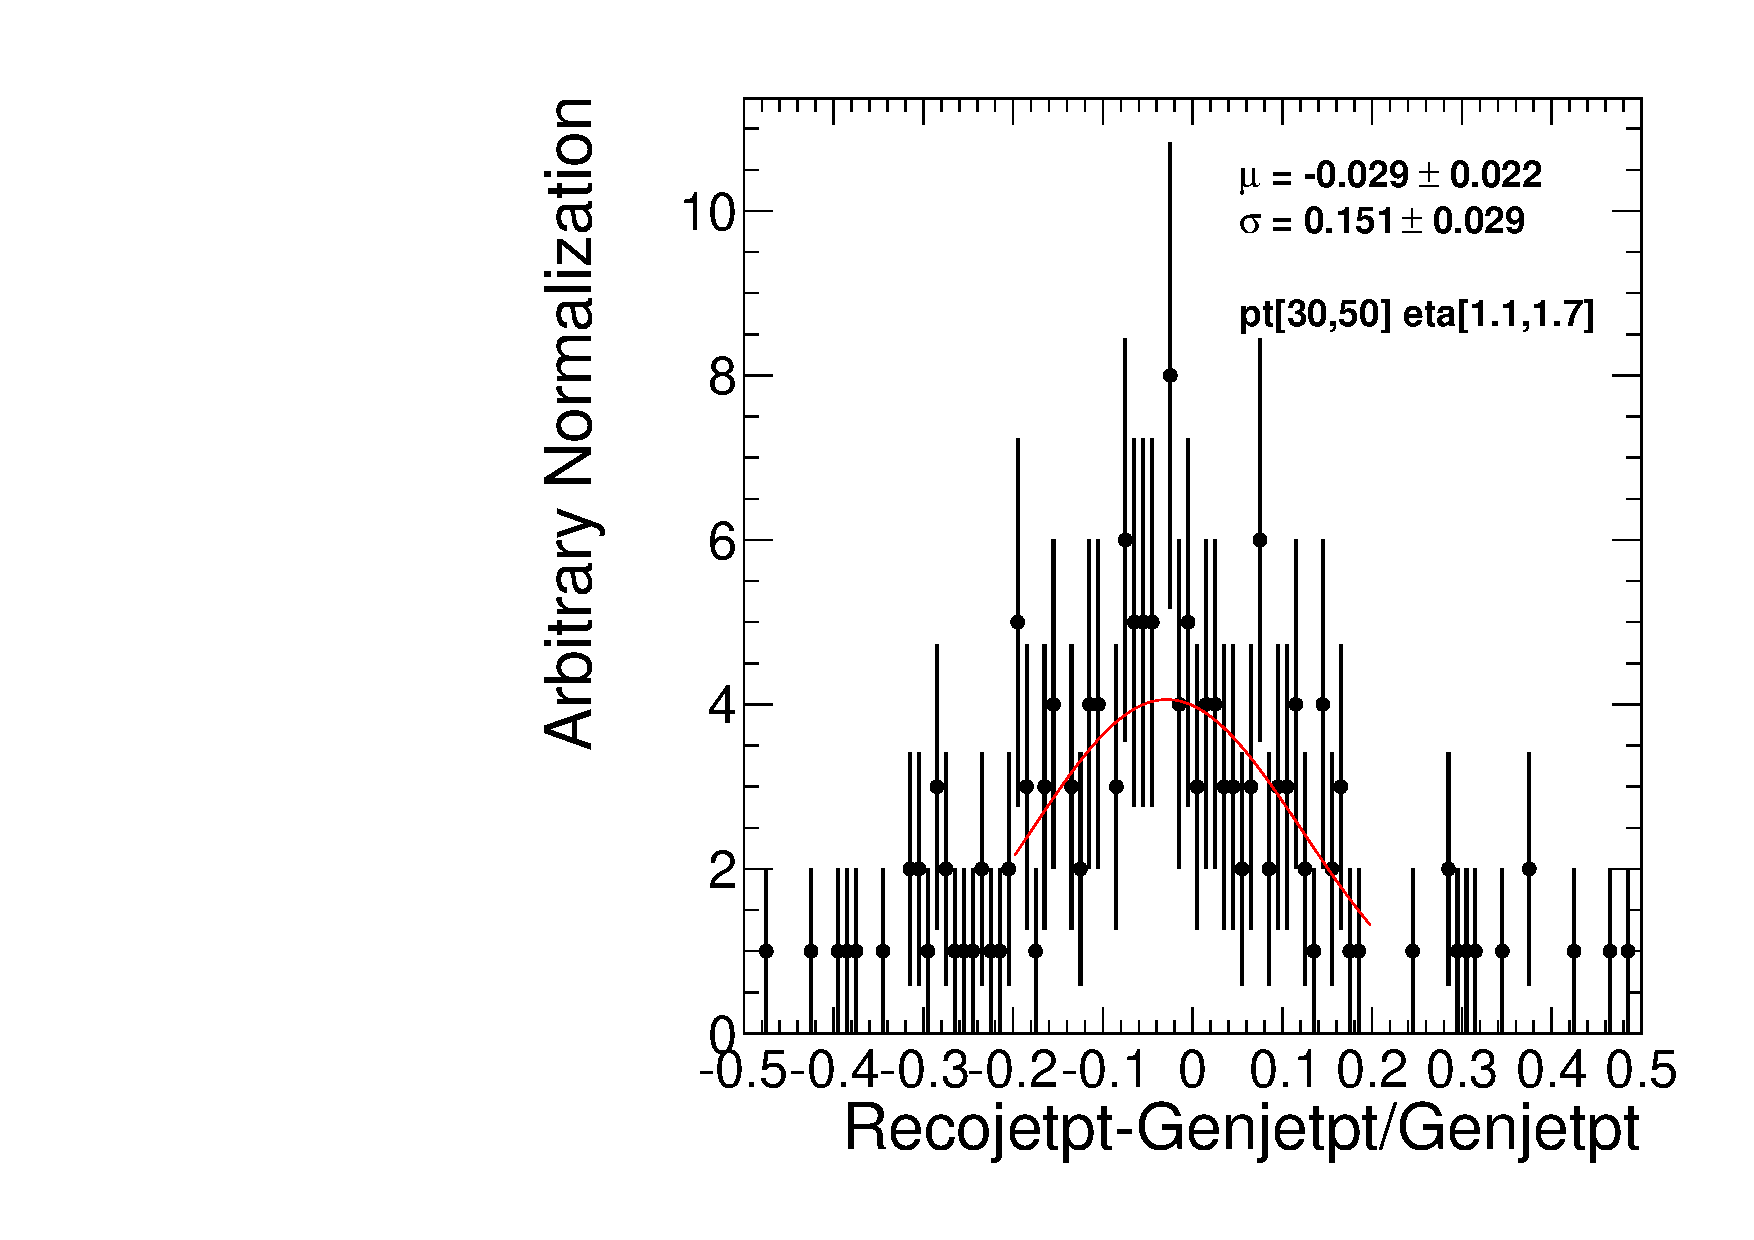
\includegraphics[width=0.45\textwidth]{figs/jer/mu_Recojetpt_Genjetpt_Genjetpt_1_1_1_7_30_50_tagjetresolution_jetresolution.pdf}
\put(-0.80,0.0){(a)}
\unitlength=0.33\linewidth
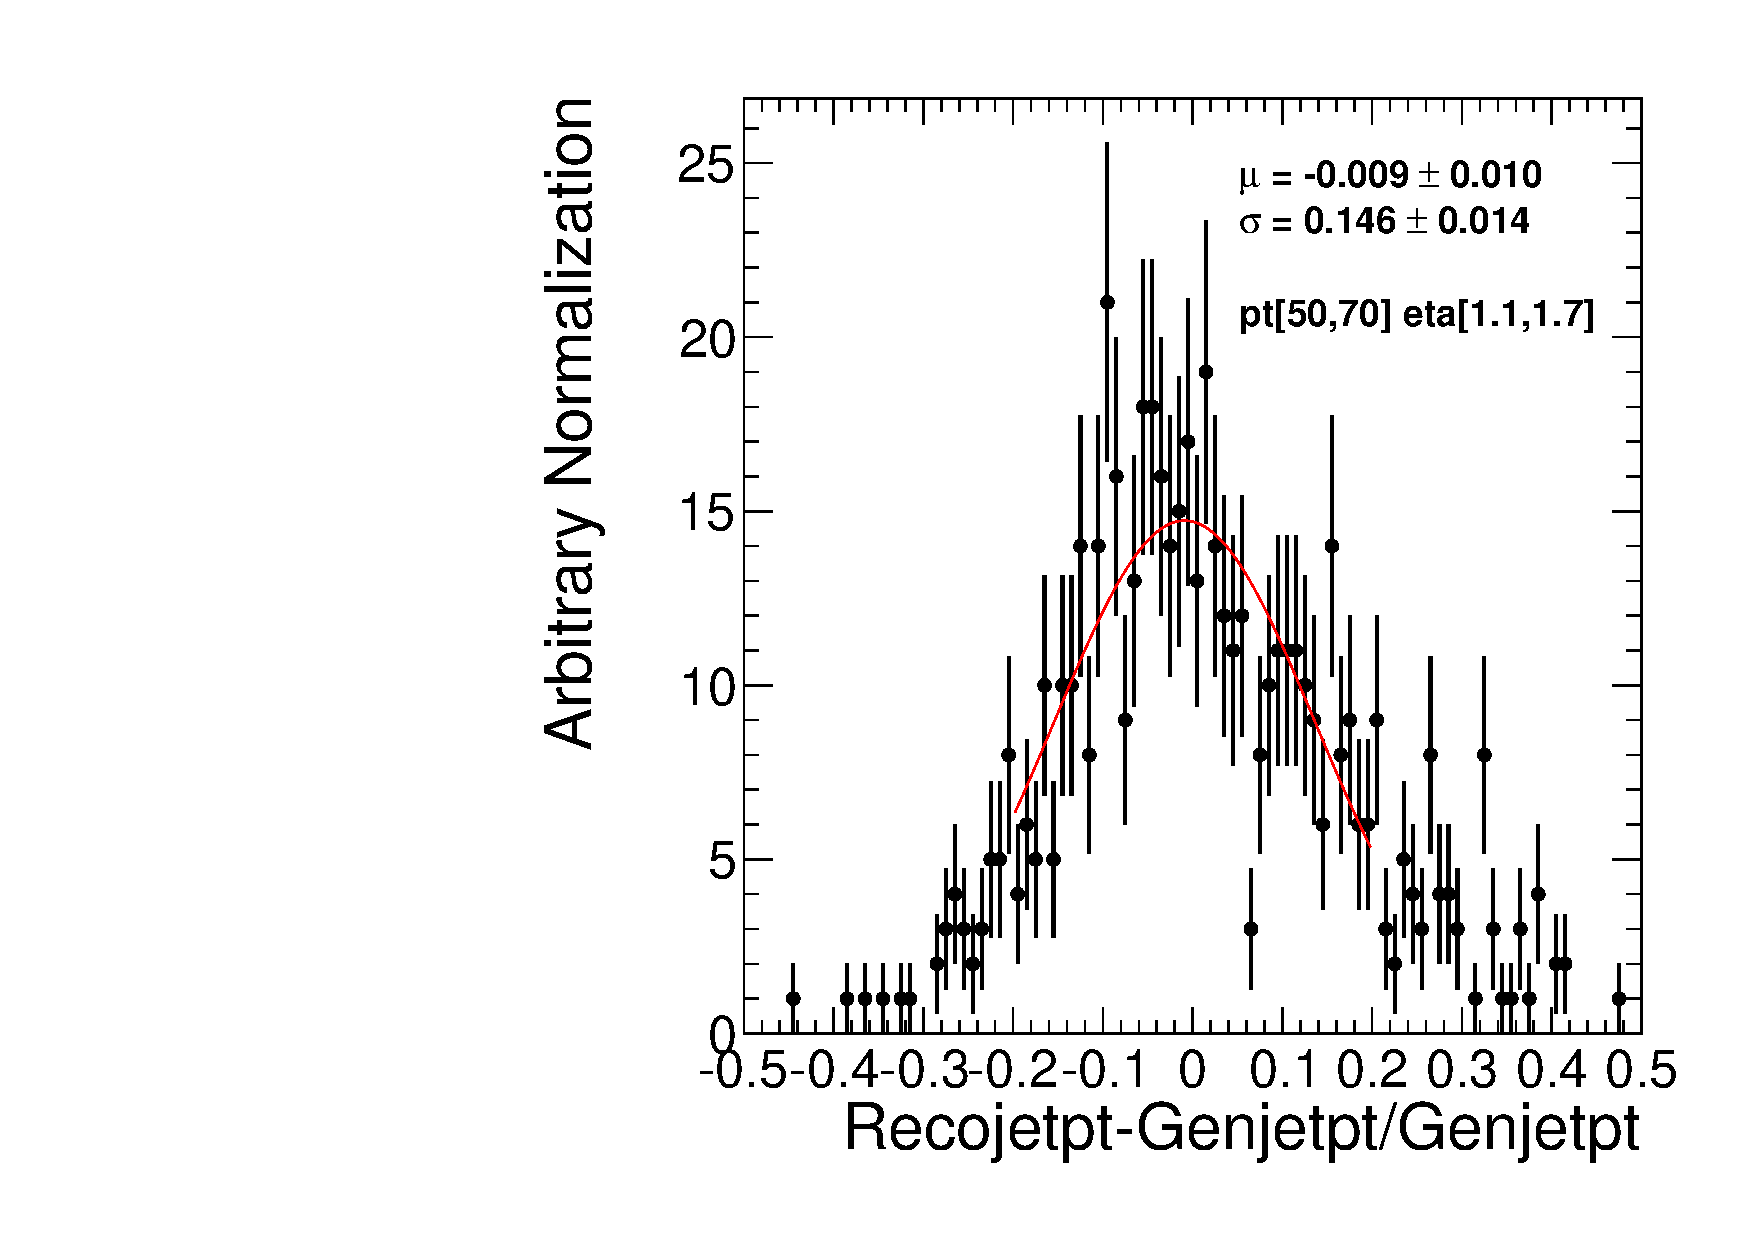
\includegraphics[width=0.45\textwidth]{figs/jer/mu_Recojetpt_Genjetpt_Genjetpt_1_1_1_7_50_70_tagjetresolution_jetresolution.pdf}
\put(-0.80,0.0){(b)} \\  
\unitlength=0.33\linewidth
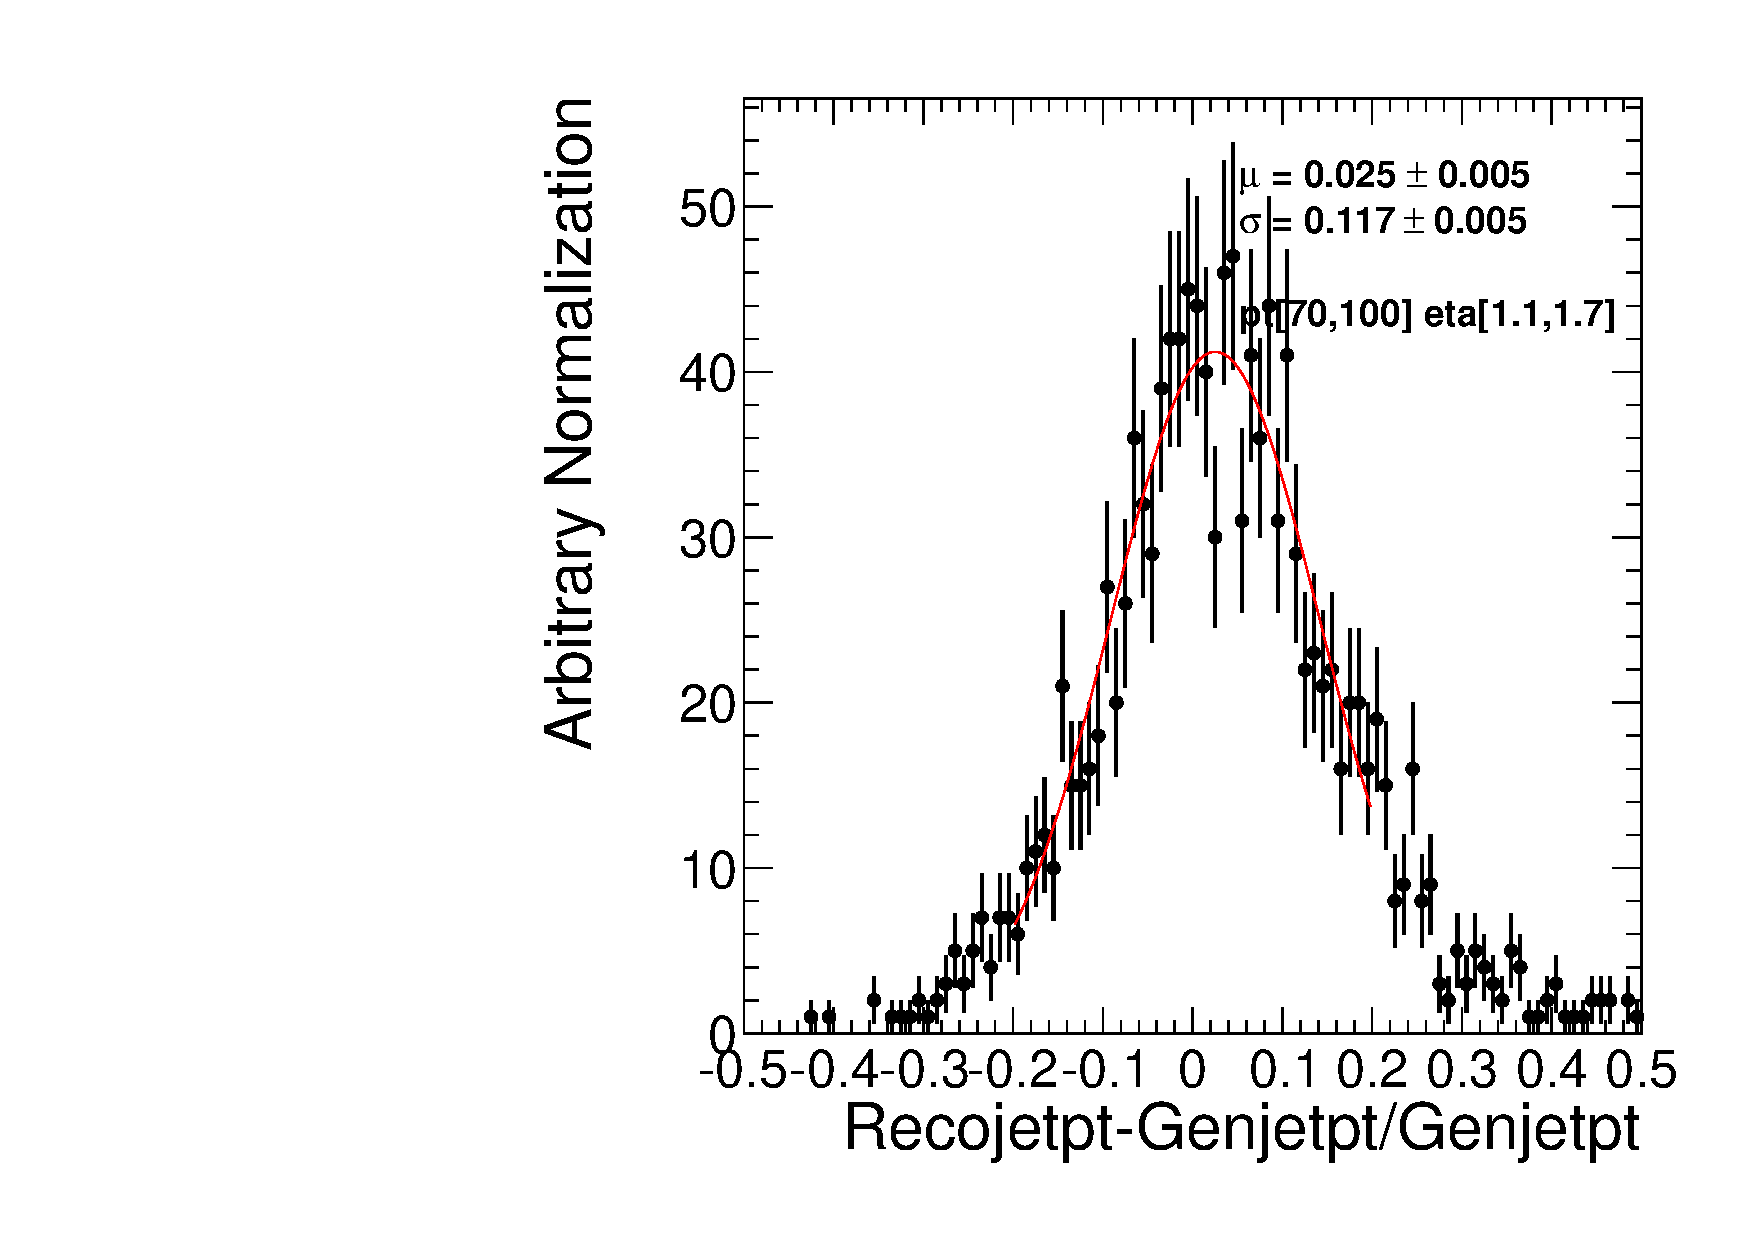
\includegraphics[width=0.45\textwidth]{figs/jer/mu_Recojetpt_Genjetpt_Genjetpt_1_1_1_7_70_100_tagjetresolution_jetresolution.pdf}
\put(-0.80,0.0){(c)}
\unitlength=0.33\linewidth
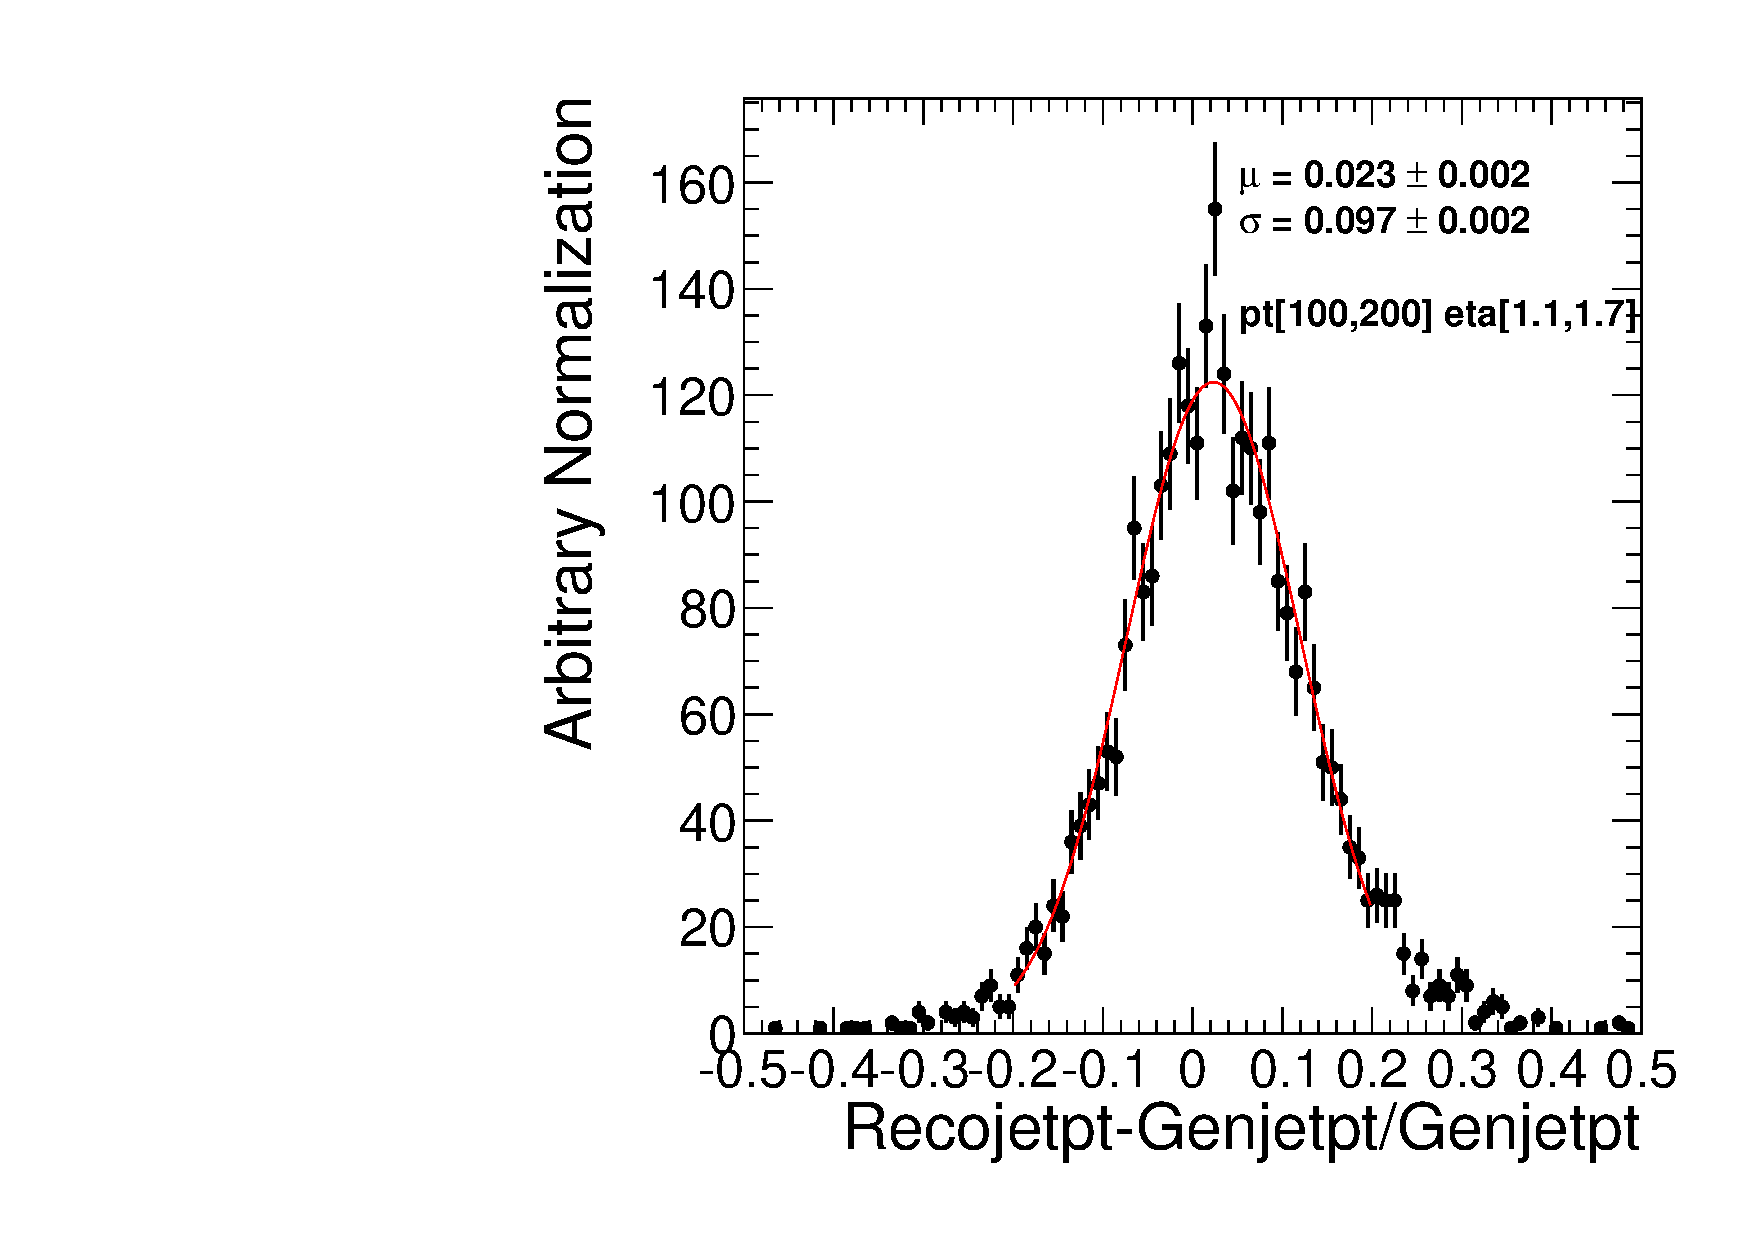
\includegraphics[width=0.45\textwidth]{figs/jer/mu_Recojetpt_Genjetpt_Genjetpt_1_1_1_7_100_200_tagjetresolution_jetresolution.pdf}
\put(-0.80,0.0){(d)}\\ 
\unitlength=0.33\linewidth
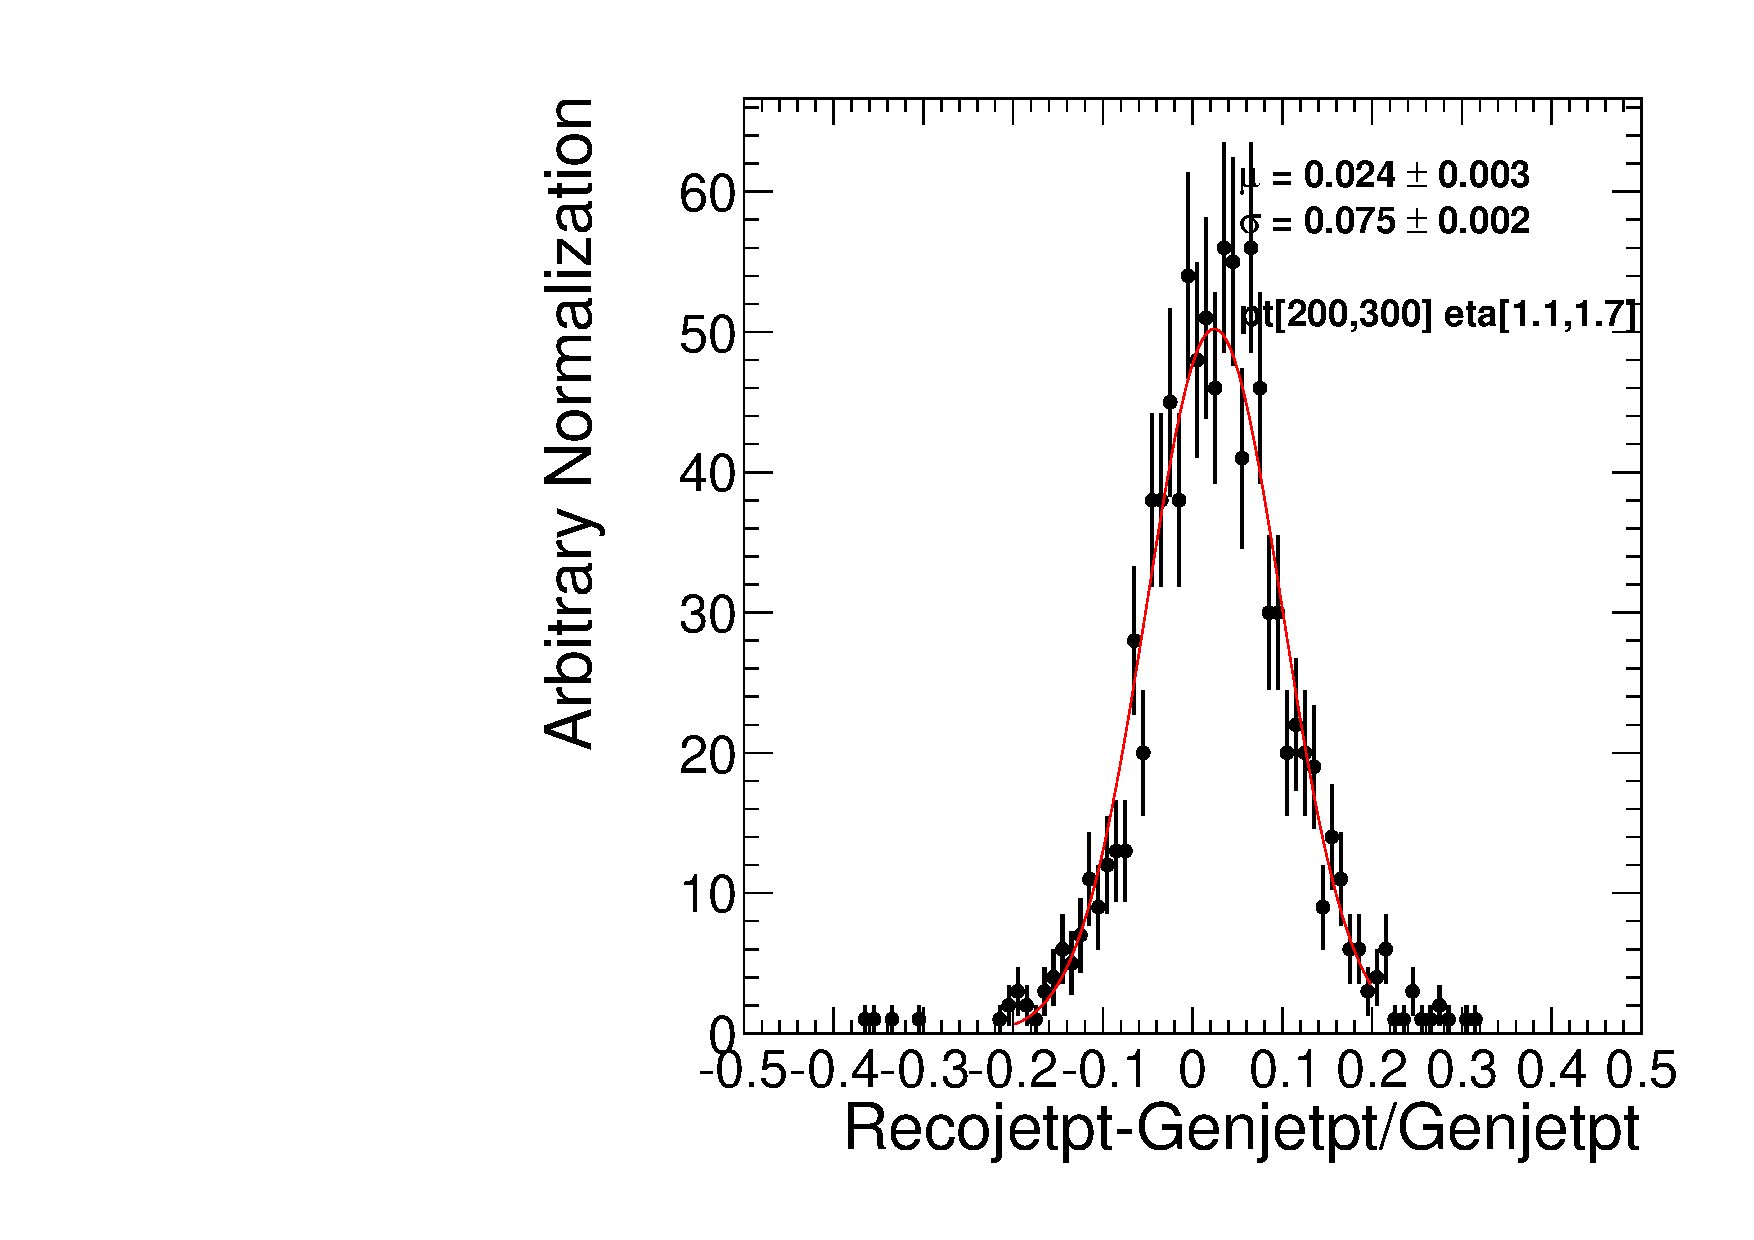
\includegraphics[width=0.45\textwidth]{figs/jer/mu_Recojetpt_Genjetpt_Genjetpt_1_1_1_7_200_300_tagjetresolution_jetresolution.pdf}
\put(-0.80,0.0){(e)} 
\unitlength=0.33\linewidth
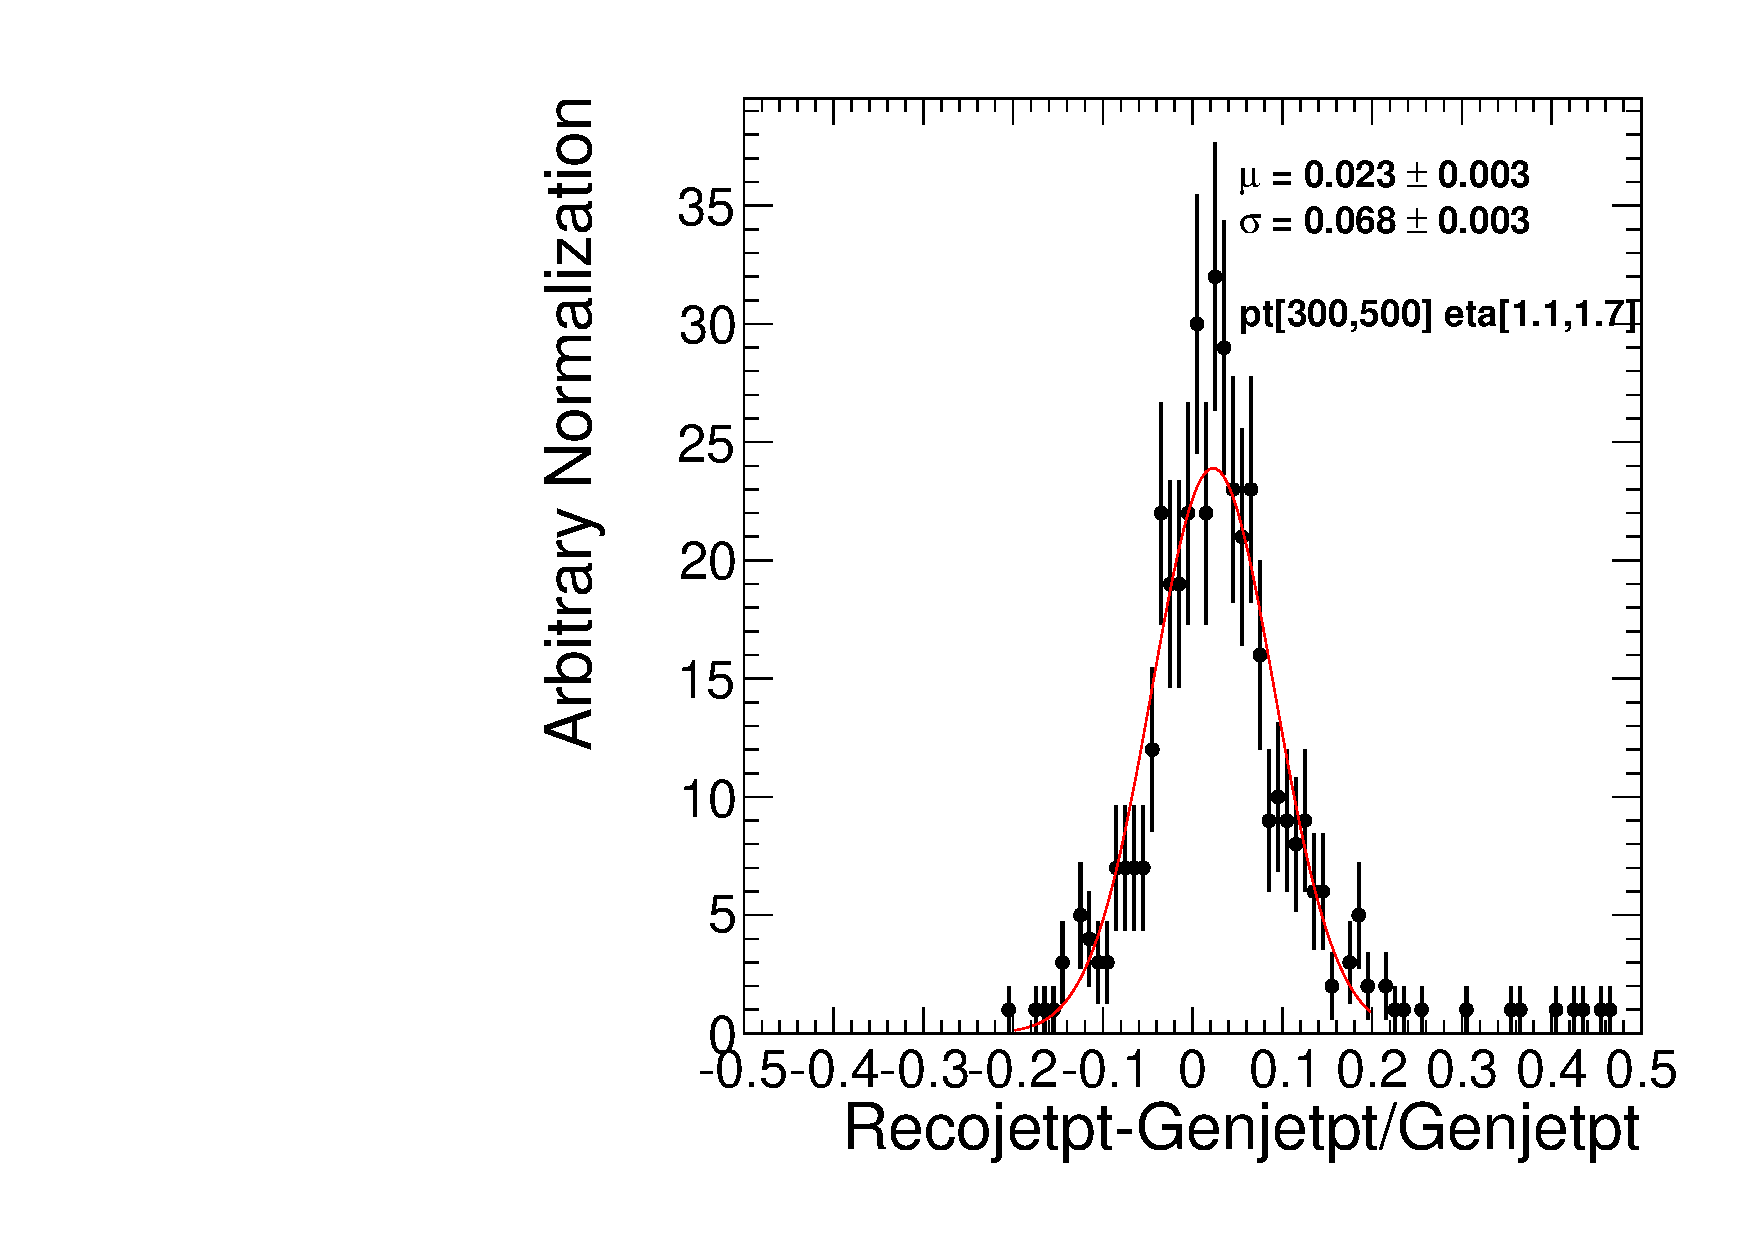
\includegraphics[width=0.45\textwidth]{figs/jer/mu_Recojetpt_Genjetpt_Genjetpt_1_1_1_7_300_500_tagjetresolution_jetresolution.pdf}
\put(-0.80,0.0){(f)} 
\caption{Fit result in jet $\eta$ bin: [1.1, 1.7] for six $p_{T}$[GeV/c] bins: 
         (a) [30, 50], (b) [50, 70], (b) [70, 100], (d) [100, 200], (e) [200, 300], (f) [300, 500].}
\label{fig:jer_eta_3_pt_3}}
\end{figure}

\begin{figure}[ht]{\centering
\unitlength=0.33\linewidth
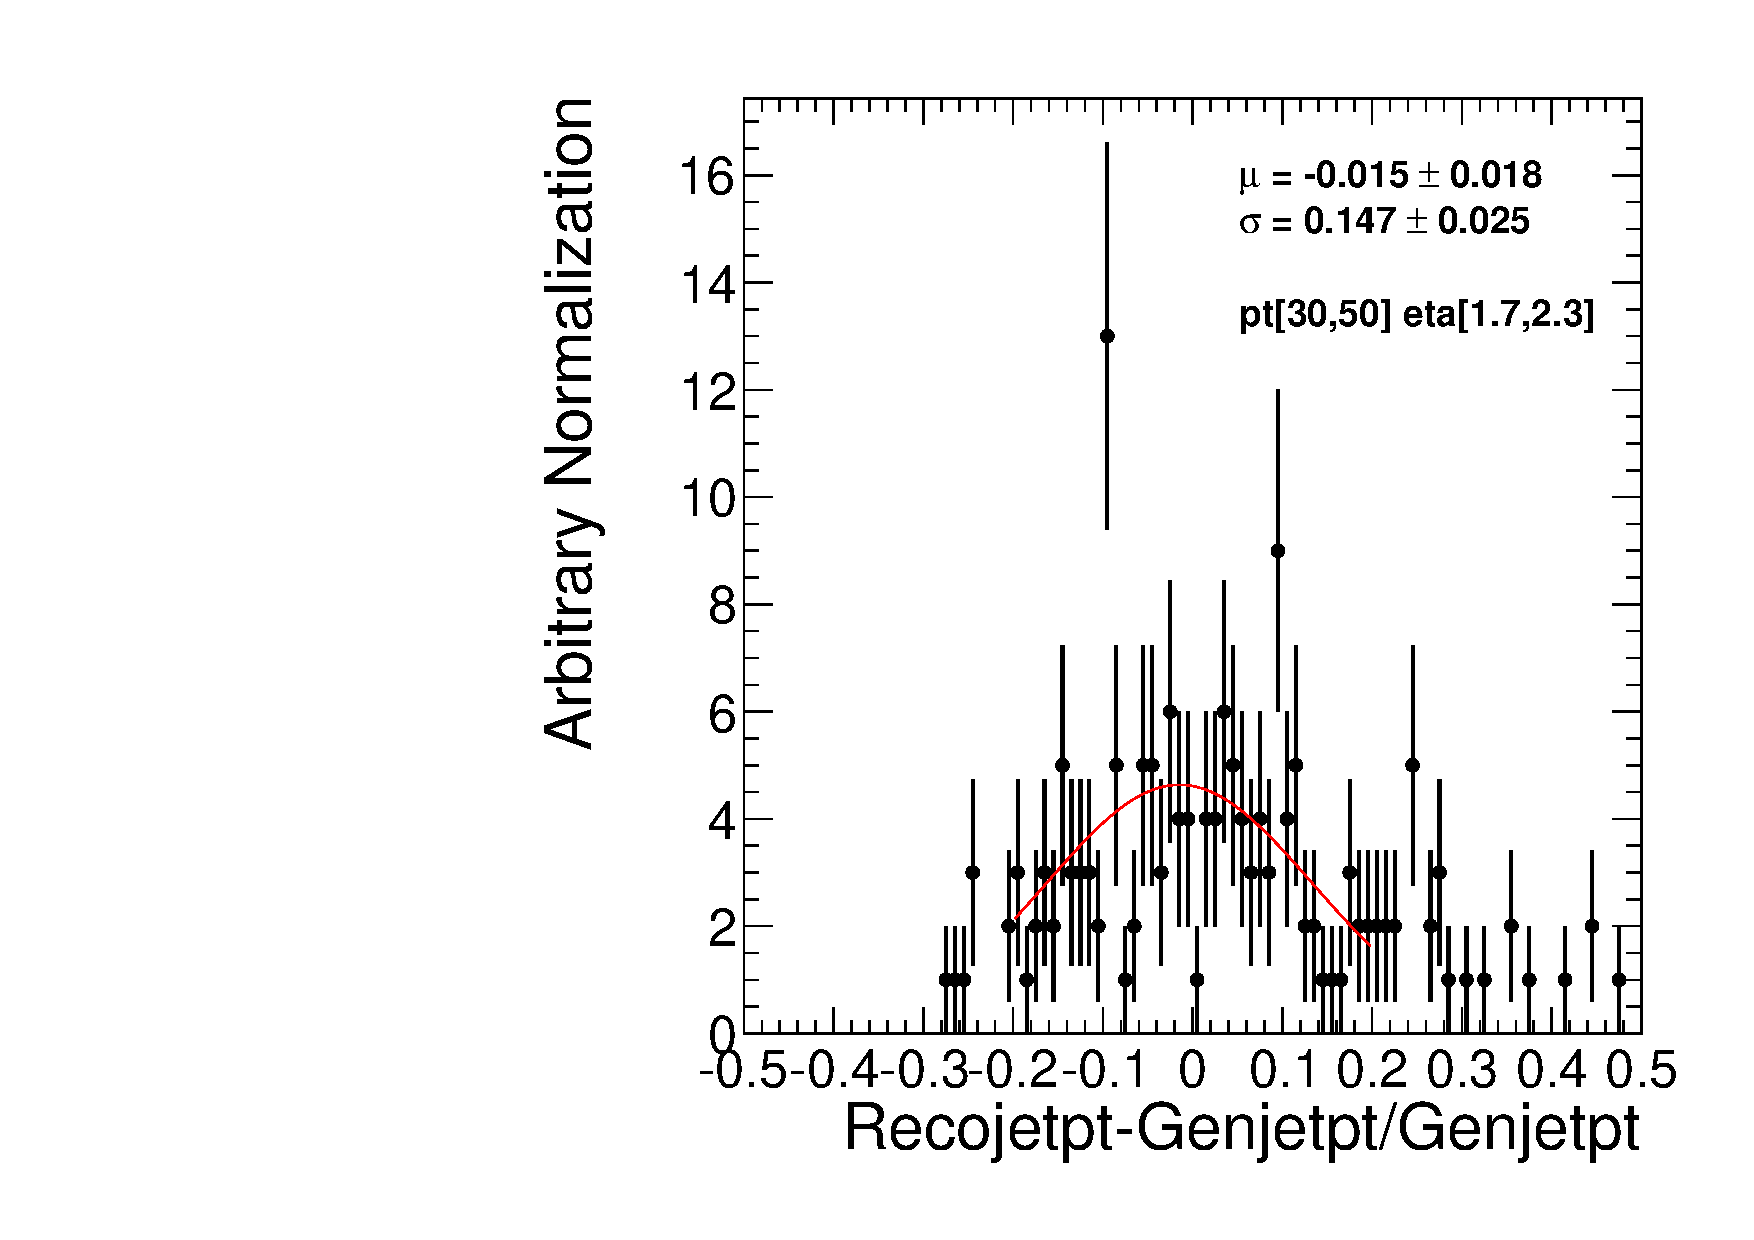
\includegraphics[width=0.45\textwidth]{figs/jer/mu_Recojetpt_Genjetpt_Genjetpt_1_7_2_3_30_50_tagjetresolution_jetresolution.pdf}
\put(-0.80,0.0){(a)}
\unitlength=0.33\linewidth
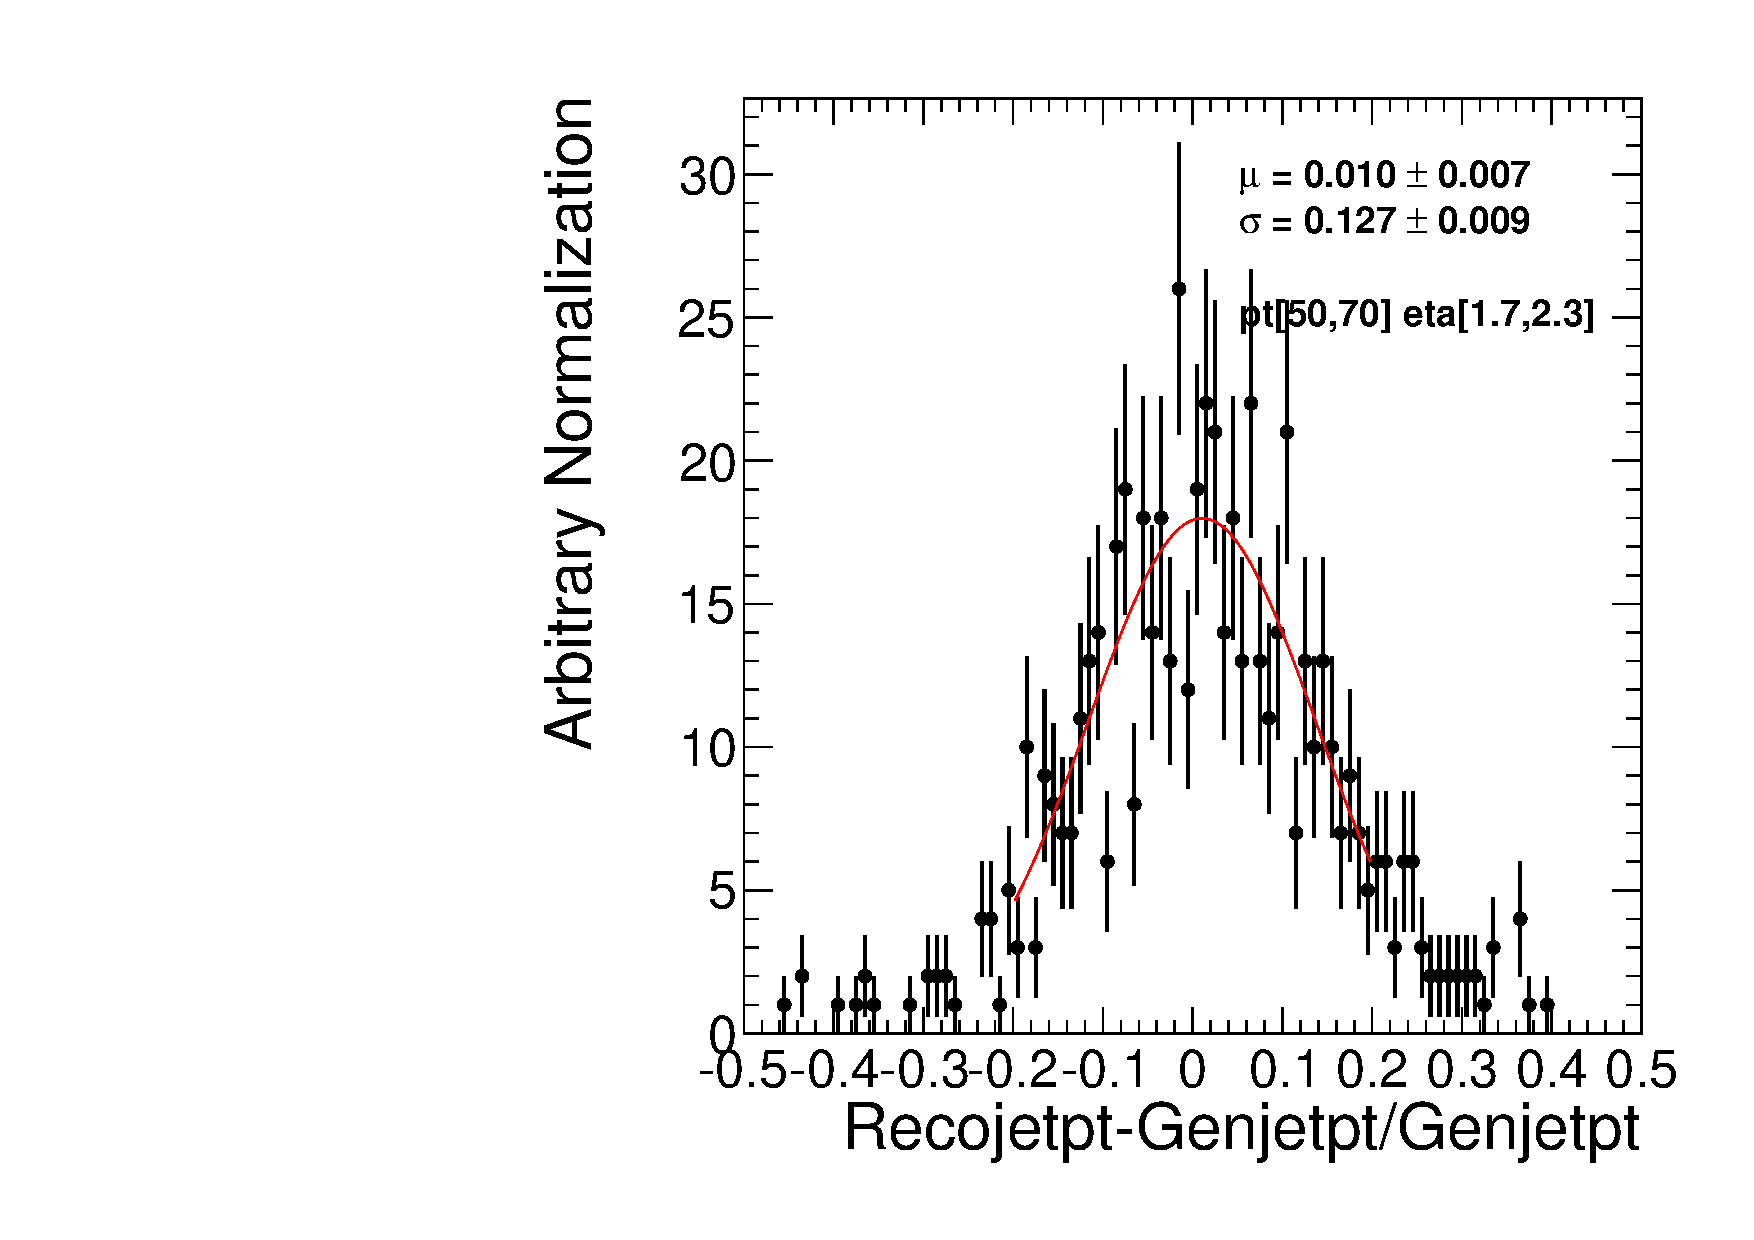
\includegraphics[width=0.45\textwidth]{figs/jer/mu_Recojetpt_Genjetpt_Genjetpt_1_7_2_3_50_70_tagjetresolution_jetresolution.pdf}
\put(-0.80,0.0){(b)} \\  
\unitlength=0.33\linewidth
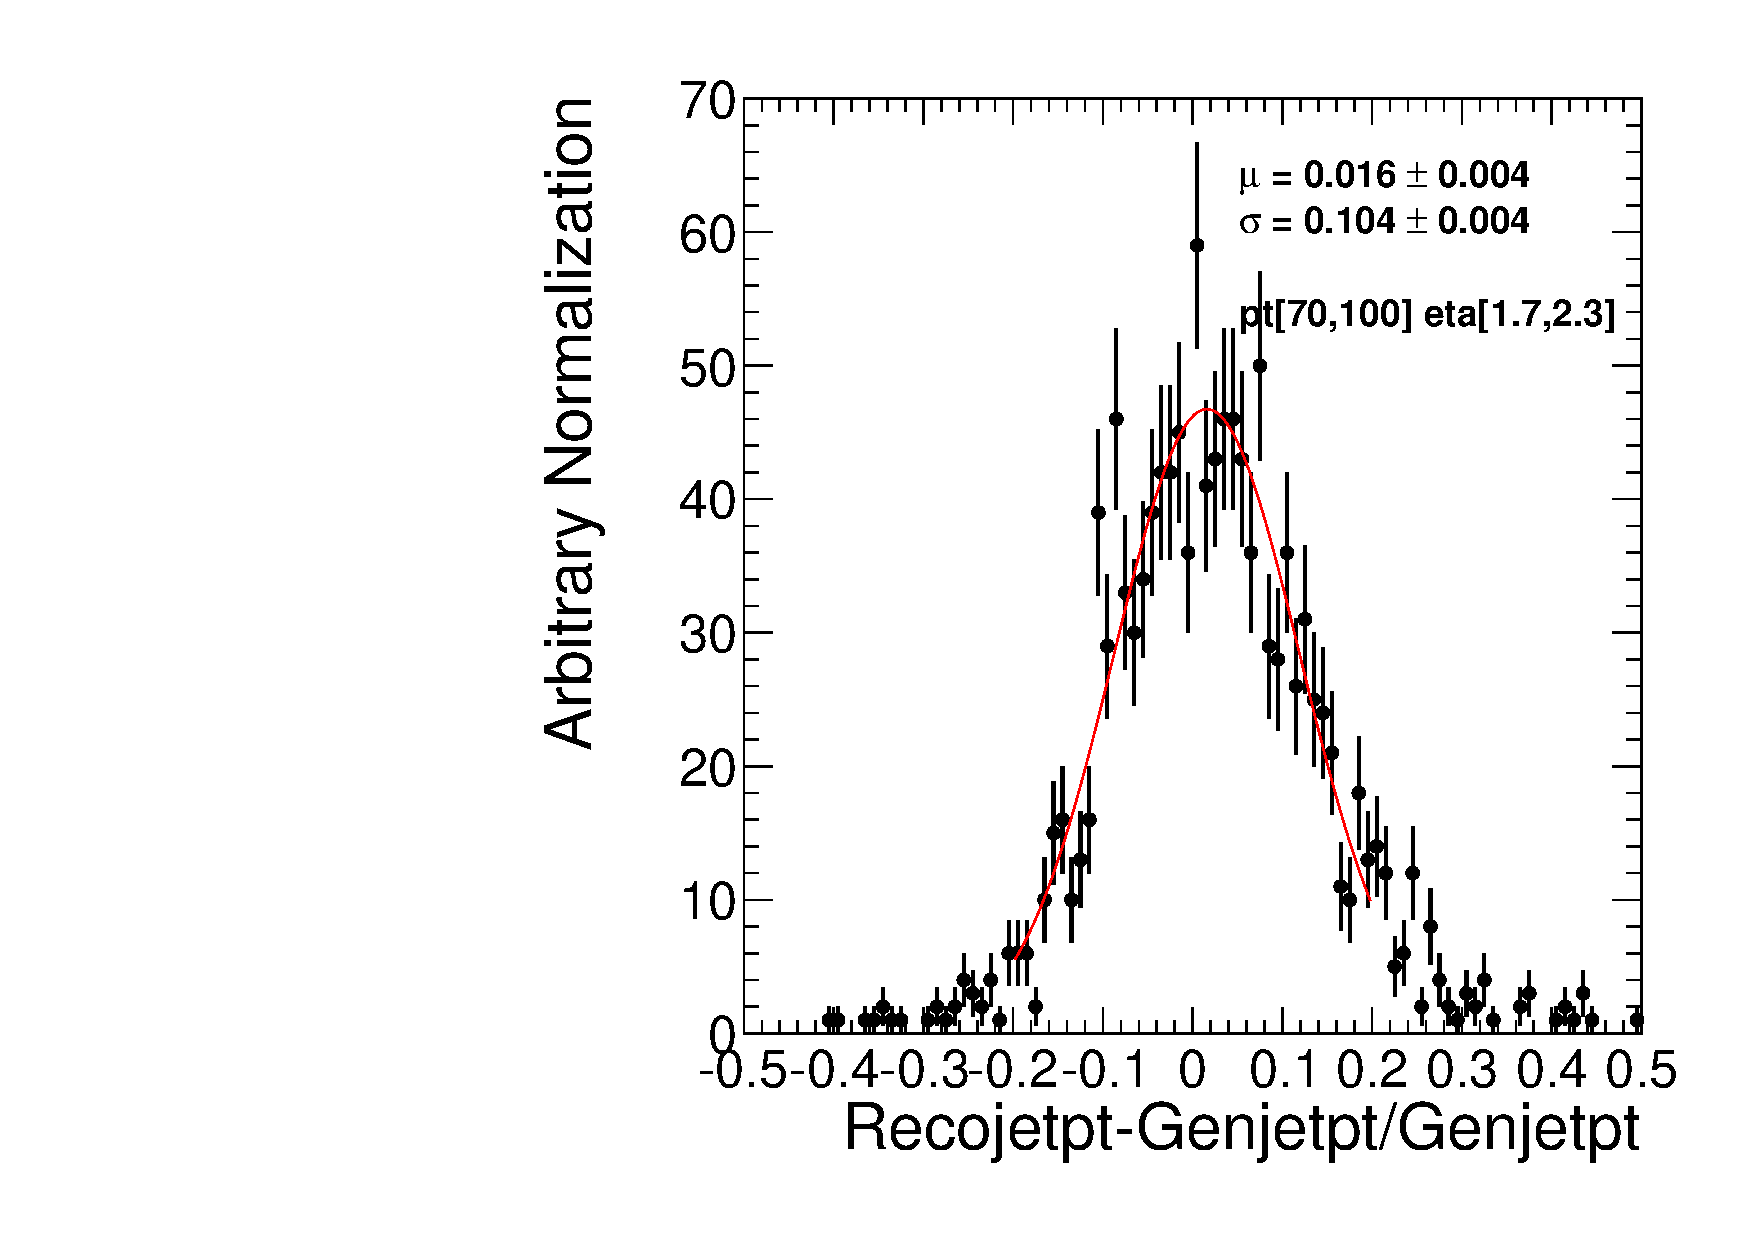
\includegraphics[width=0.45\textwidth]{figs/jer/mu_Recojetpt_Genjetpt_Genjetpt_1_7_2_3_70_100_tagjetresolution_jetresolution.pdf}
\put(-0.80,0.0){(c)}
\unitlength=0.33\linewidth
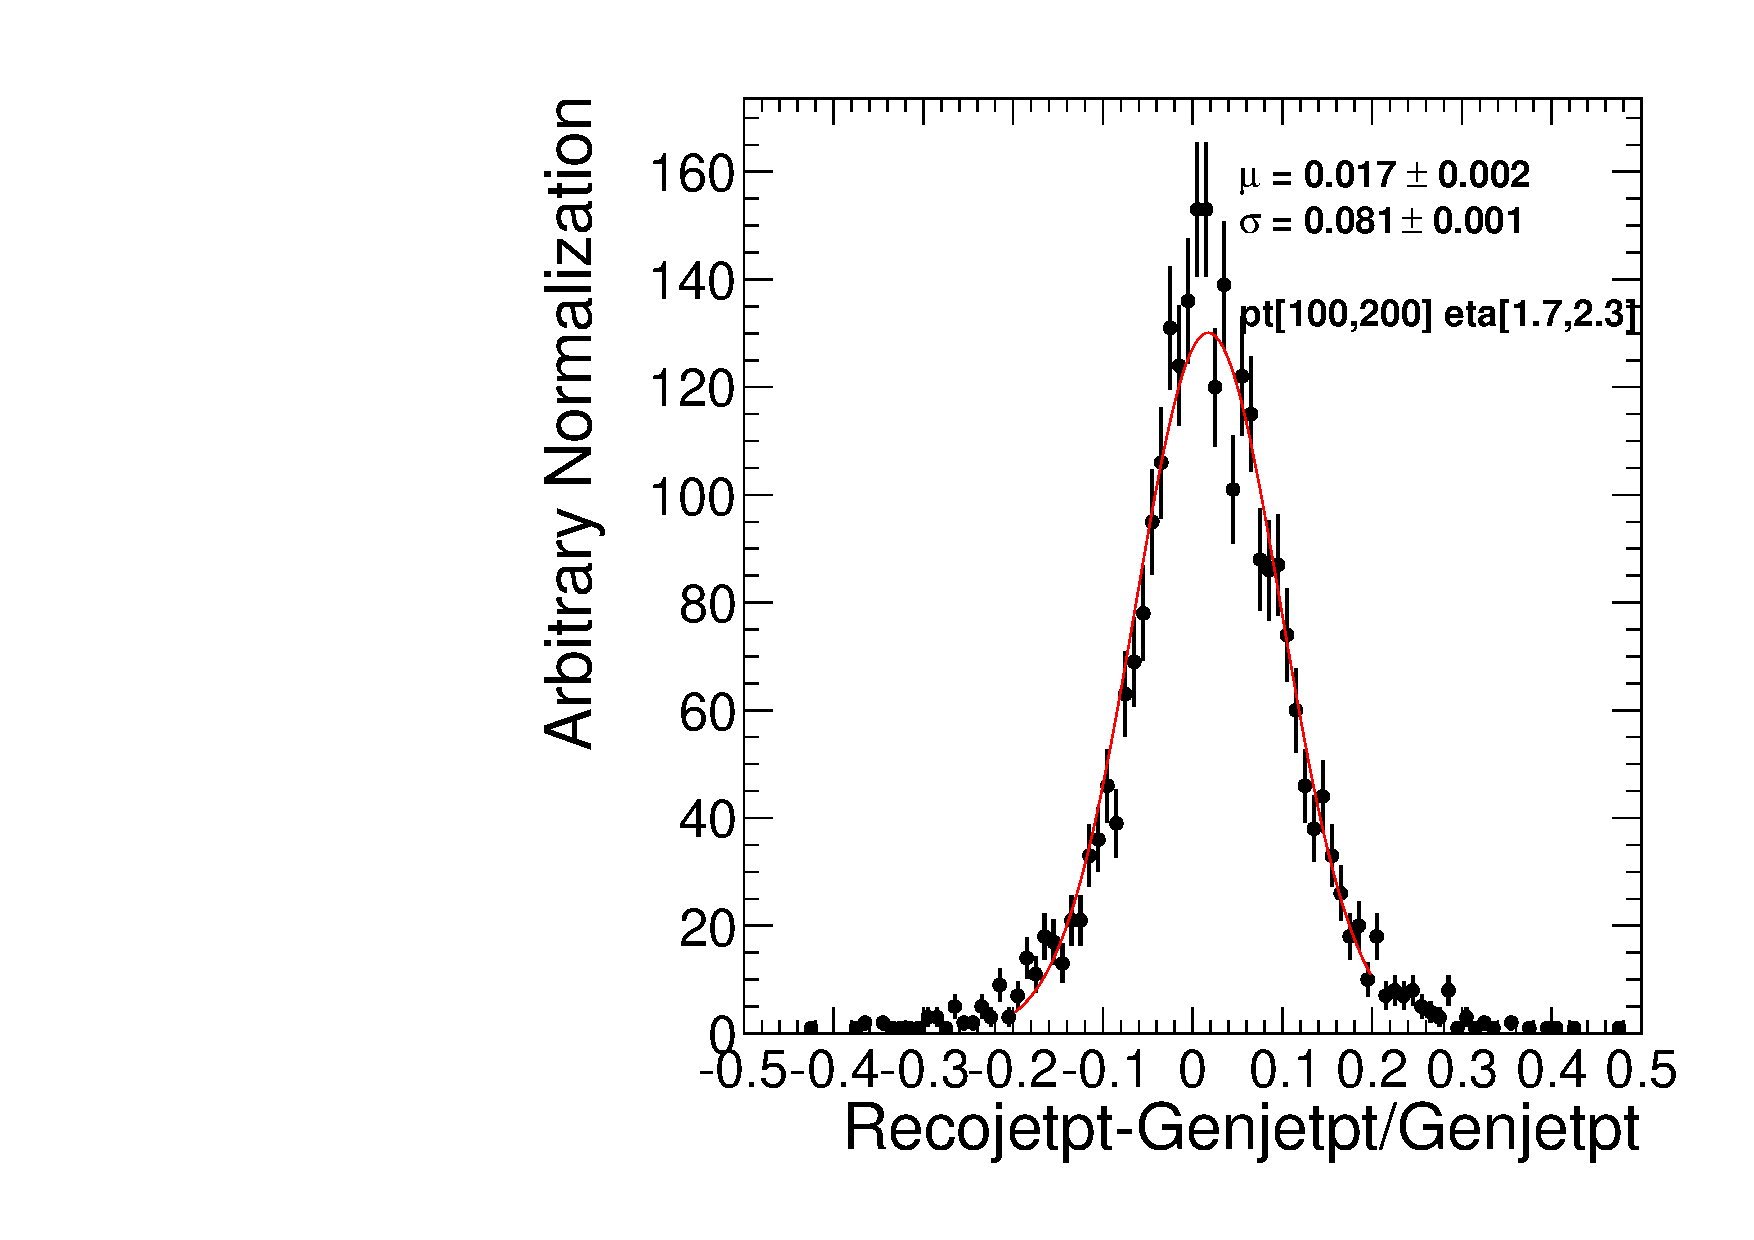
\includegraphics[width=0.45\textwidth]{figs/jer/mu_Recojetpt_Genjetpt_Genjetpt_1_7_2_3_100_200_tagjetresolution_jetresolution.pdf}
\put(-0.80,0.0){(d)}\\ 
\unitlength=0.33\linewidth
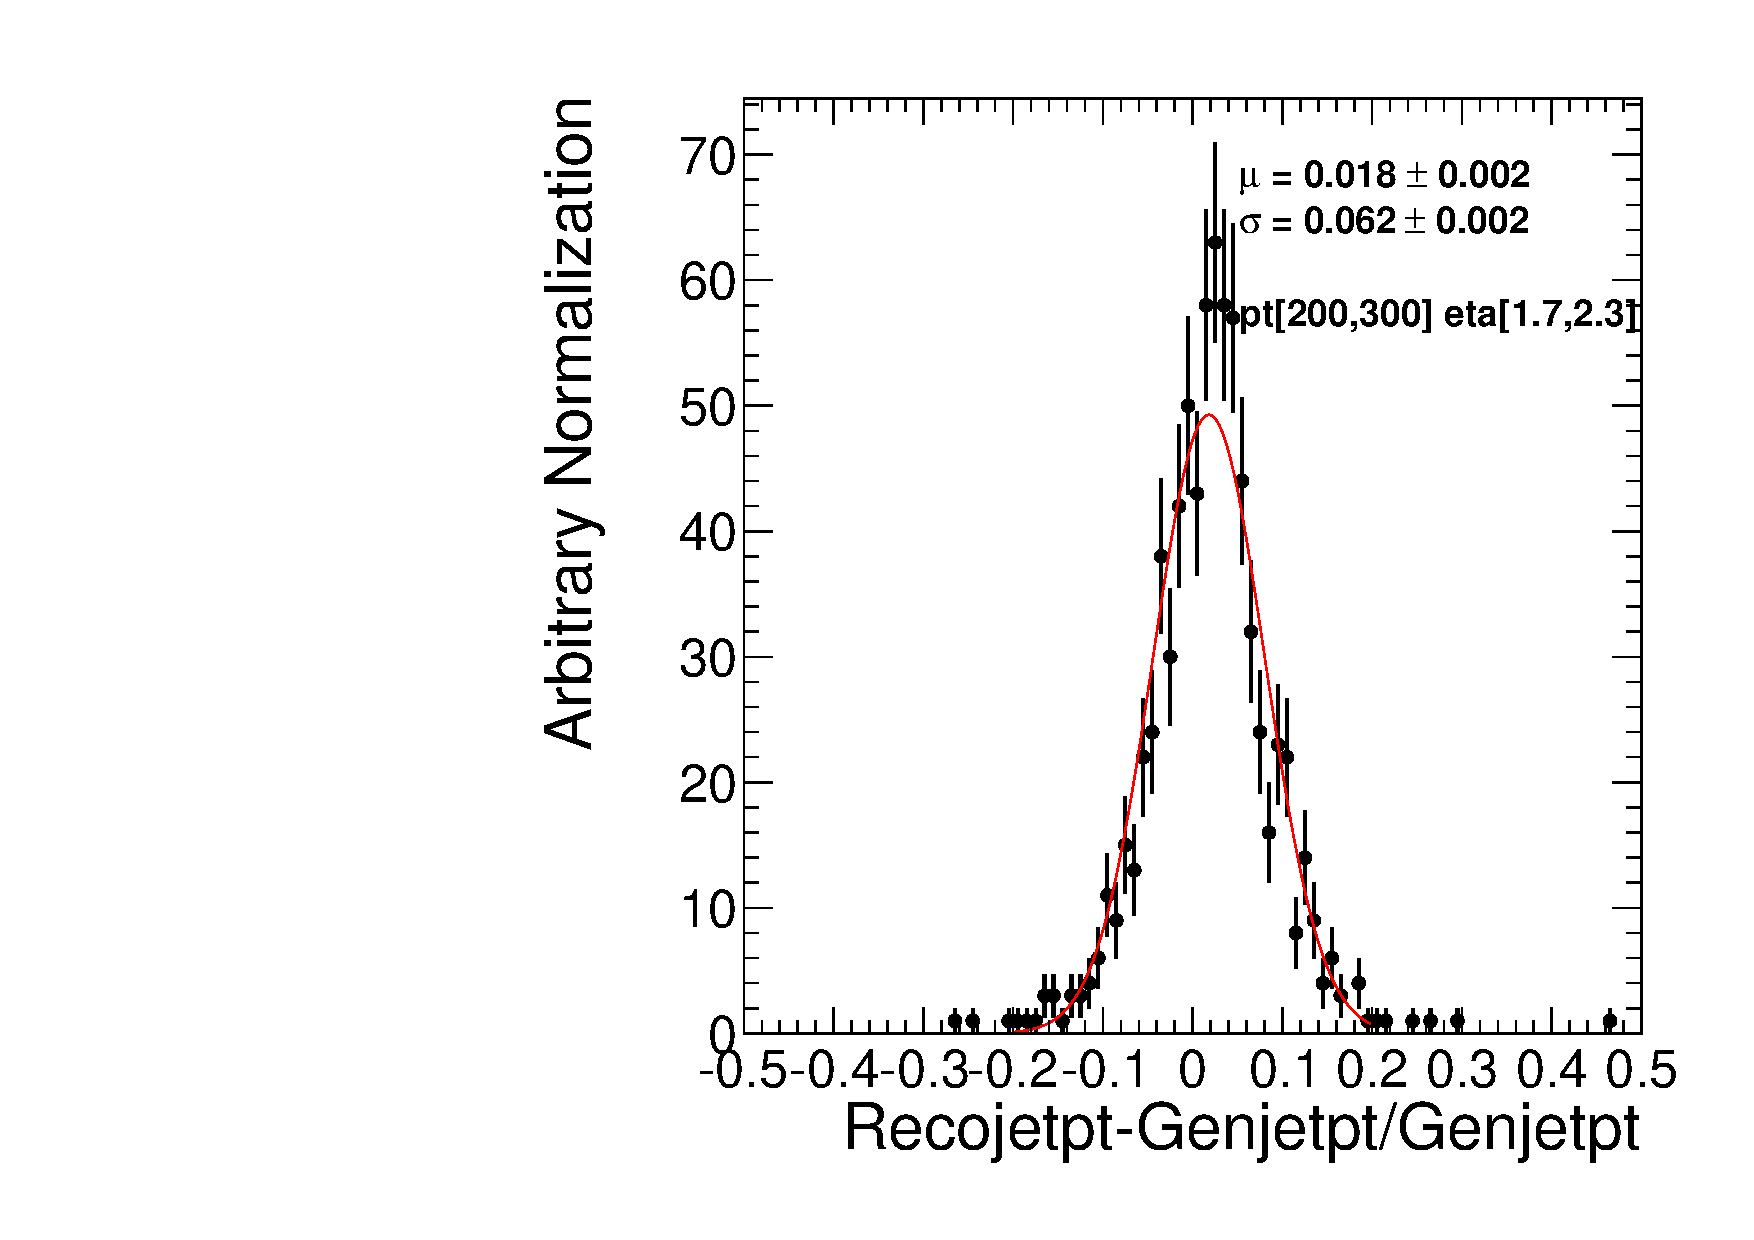
\includegraphics[width=0.45\textwidth]{figs/jer/mu_Recojetpt_Genjetpt_Genjetpt_1_7_2_3_200_300_tagjetresolution_jetresolution.pdf}
\put(-0.80,0.0){(e)} 
\unitlength=0.33\linewidth
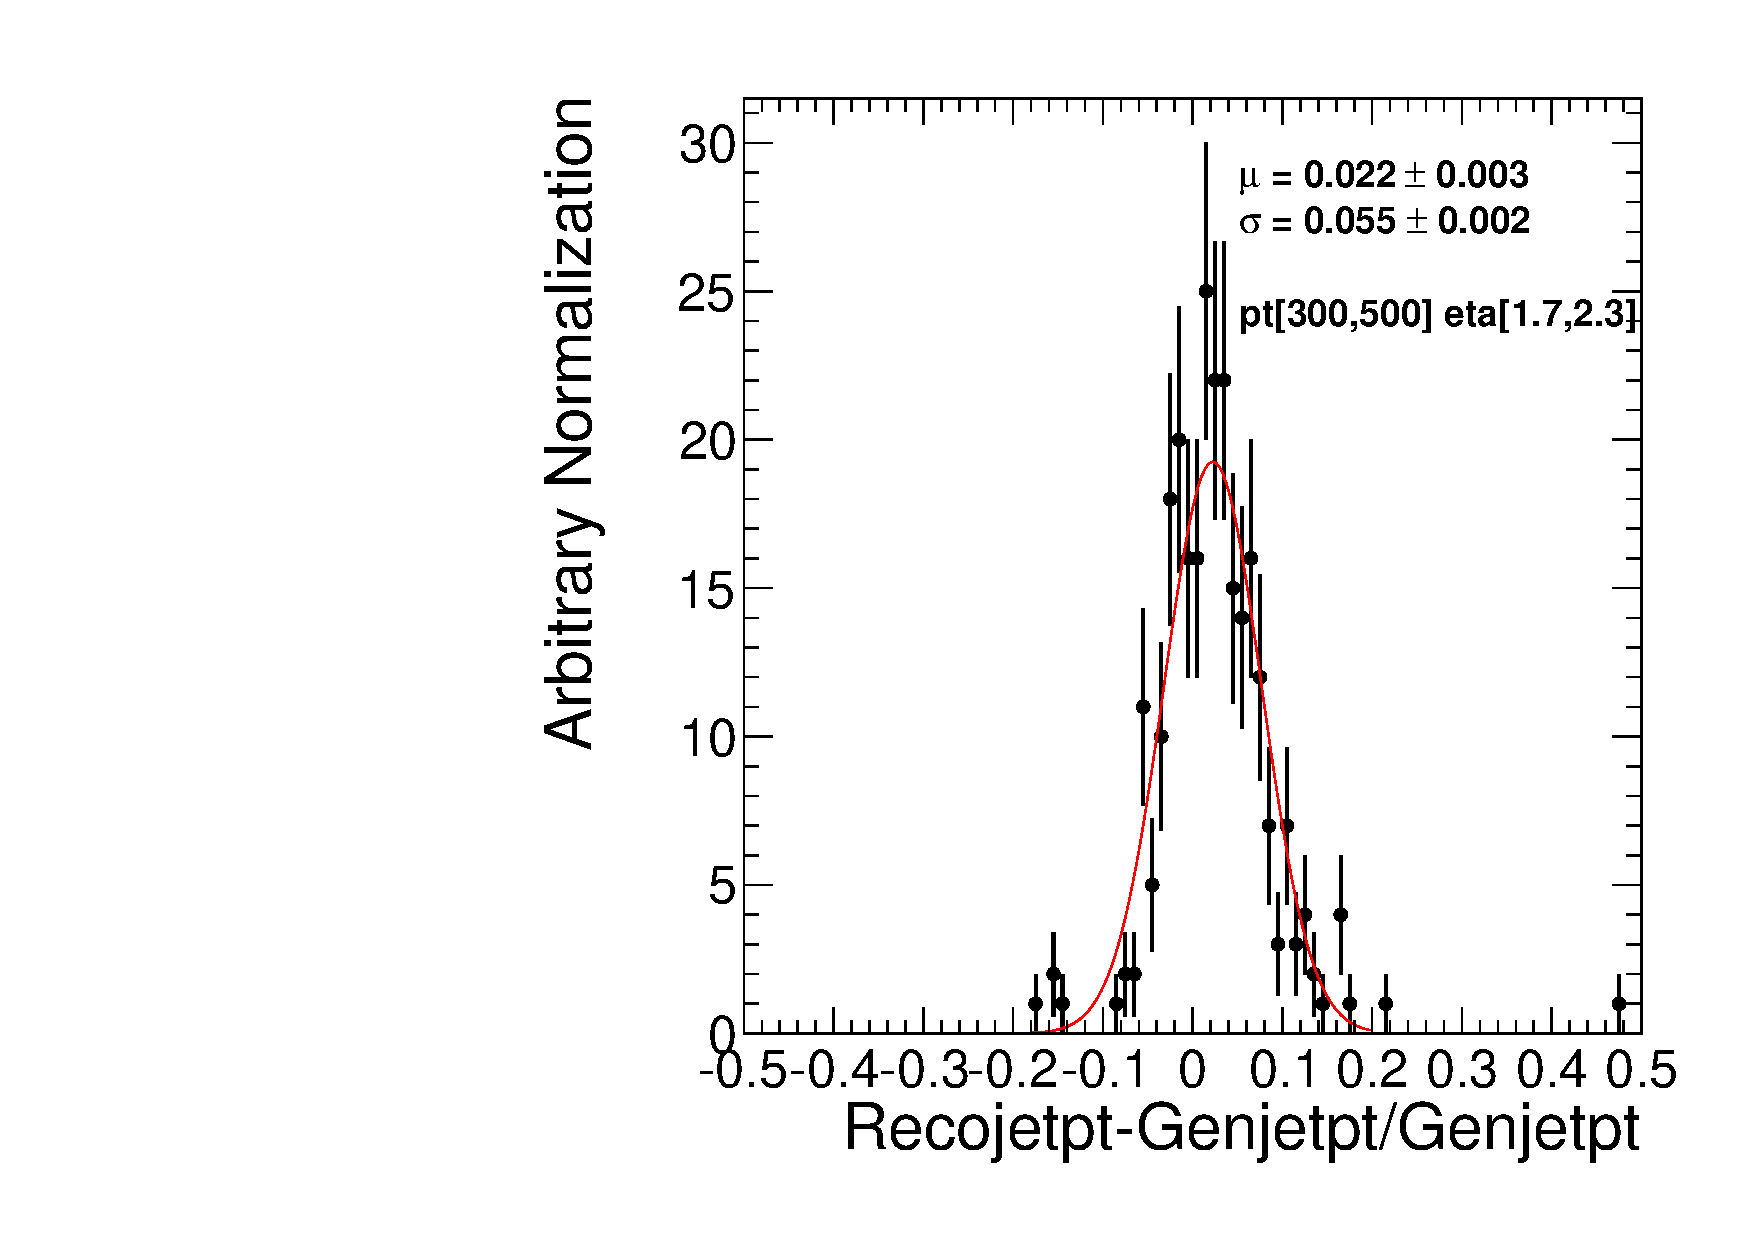
\includegraphics[width=0.45\textwidth]{figs/jer/mu_Recojetpt_Genjetpt_Genjetpt_1_7_2_3_300_500_tagjetresolution_jetresolution.pdf}
\put(-0.80,0.0){(f)} 
\caption{Fit result in jet $\eta$ bin: [1.7, 2.3] for six $p_{T}$[GeV/c] bins: 
         (a) [30, 50], (b) [50, 70], (b) [70, 100], (d) [100, 200], (e) [200, 300], (f) [300, 500].}
\label{fig:jer_eta_4_pt_4}}
\end{figure}

\begin{figure}[ht]{\centering
\unitlength=0.33\linewidth
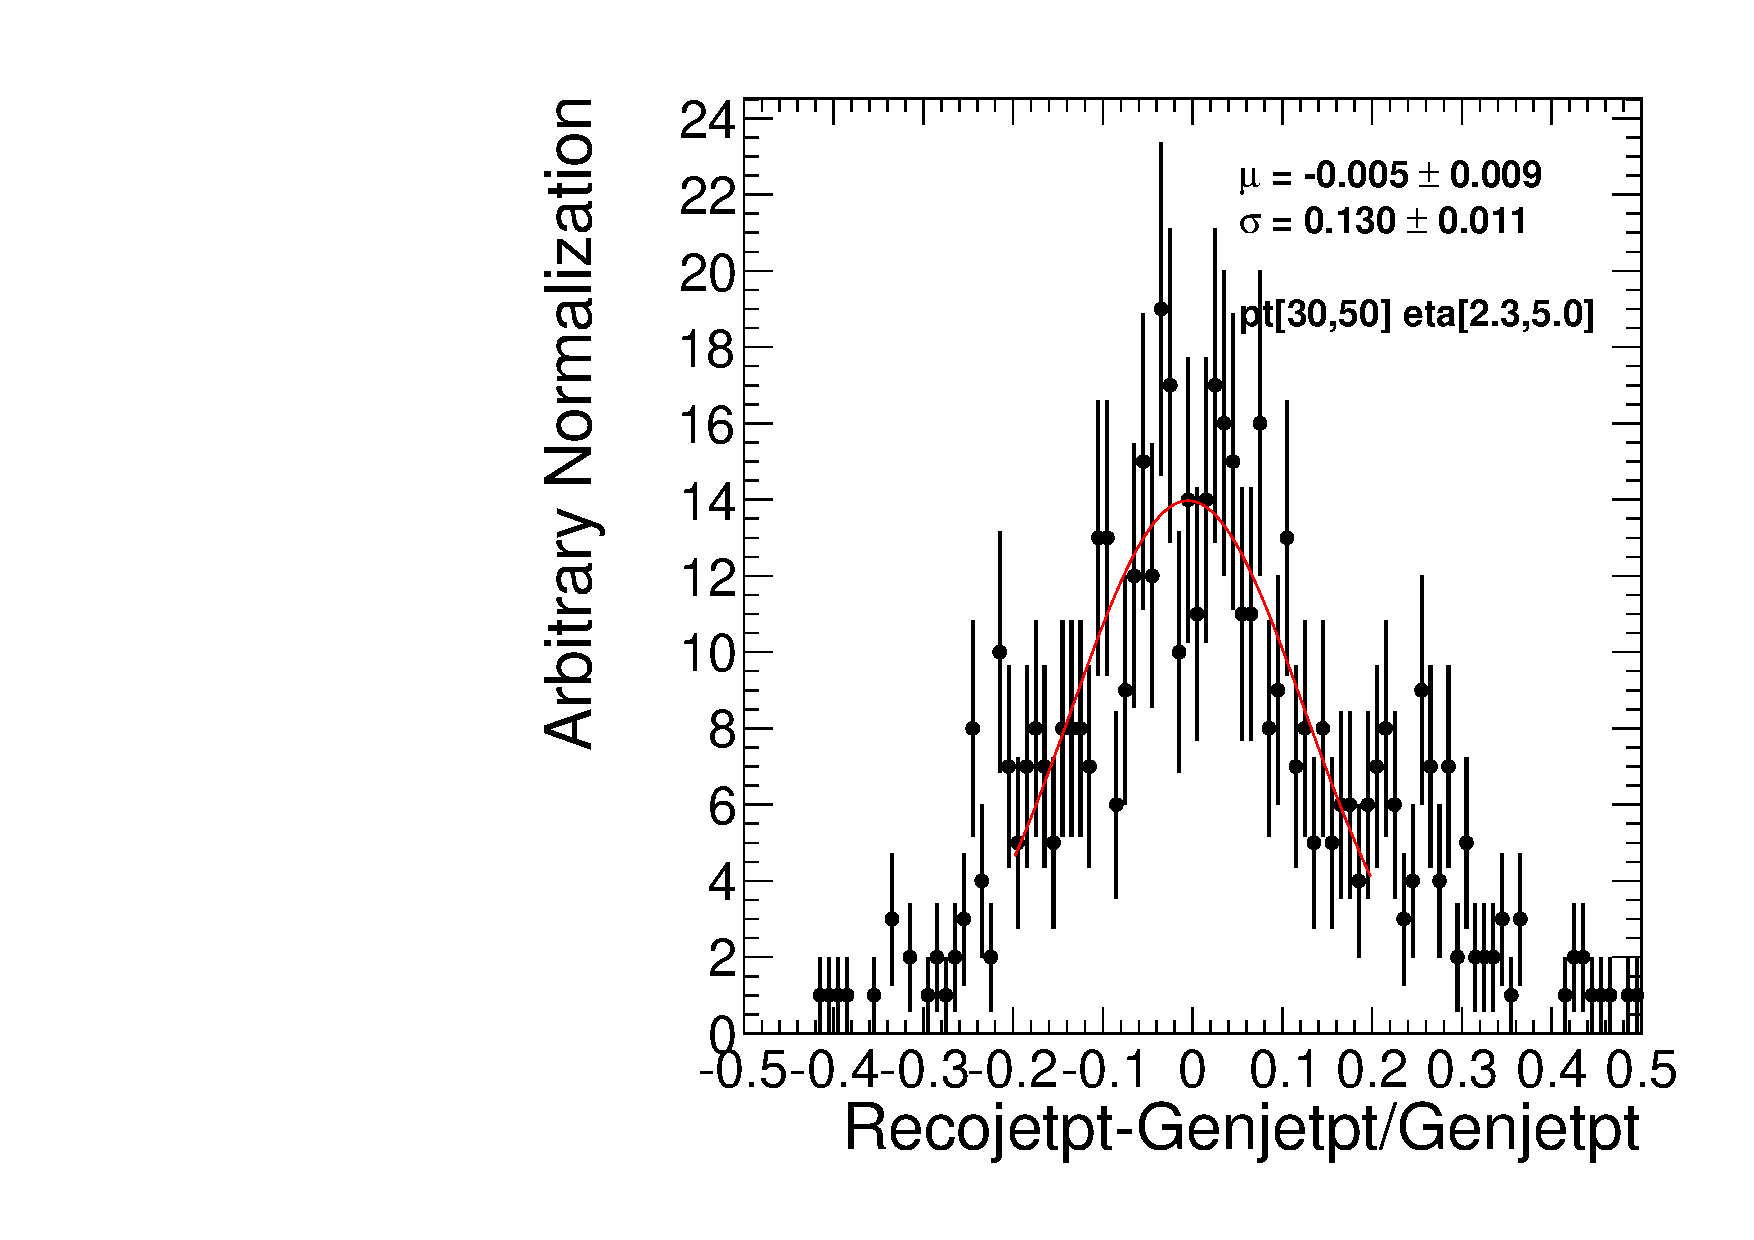
\includegraphics[width=0.45\textwidth]{figs/jer/mu_Recojetpt_Genjetpt_Genjetpt_2_3_5_0_30_50_tagjetresolution_jetresolution.pdf}
\put(-0.80,0.0){(a)}
\unitlength=0.33\linewidth
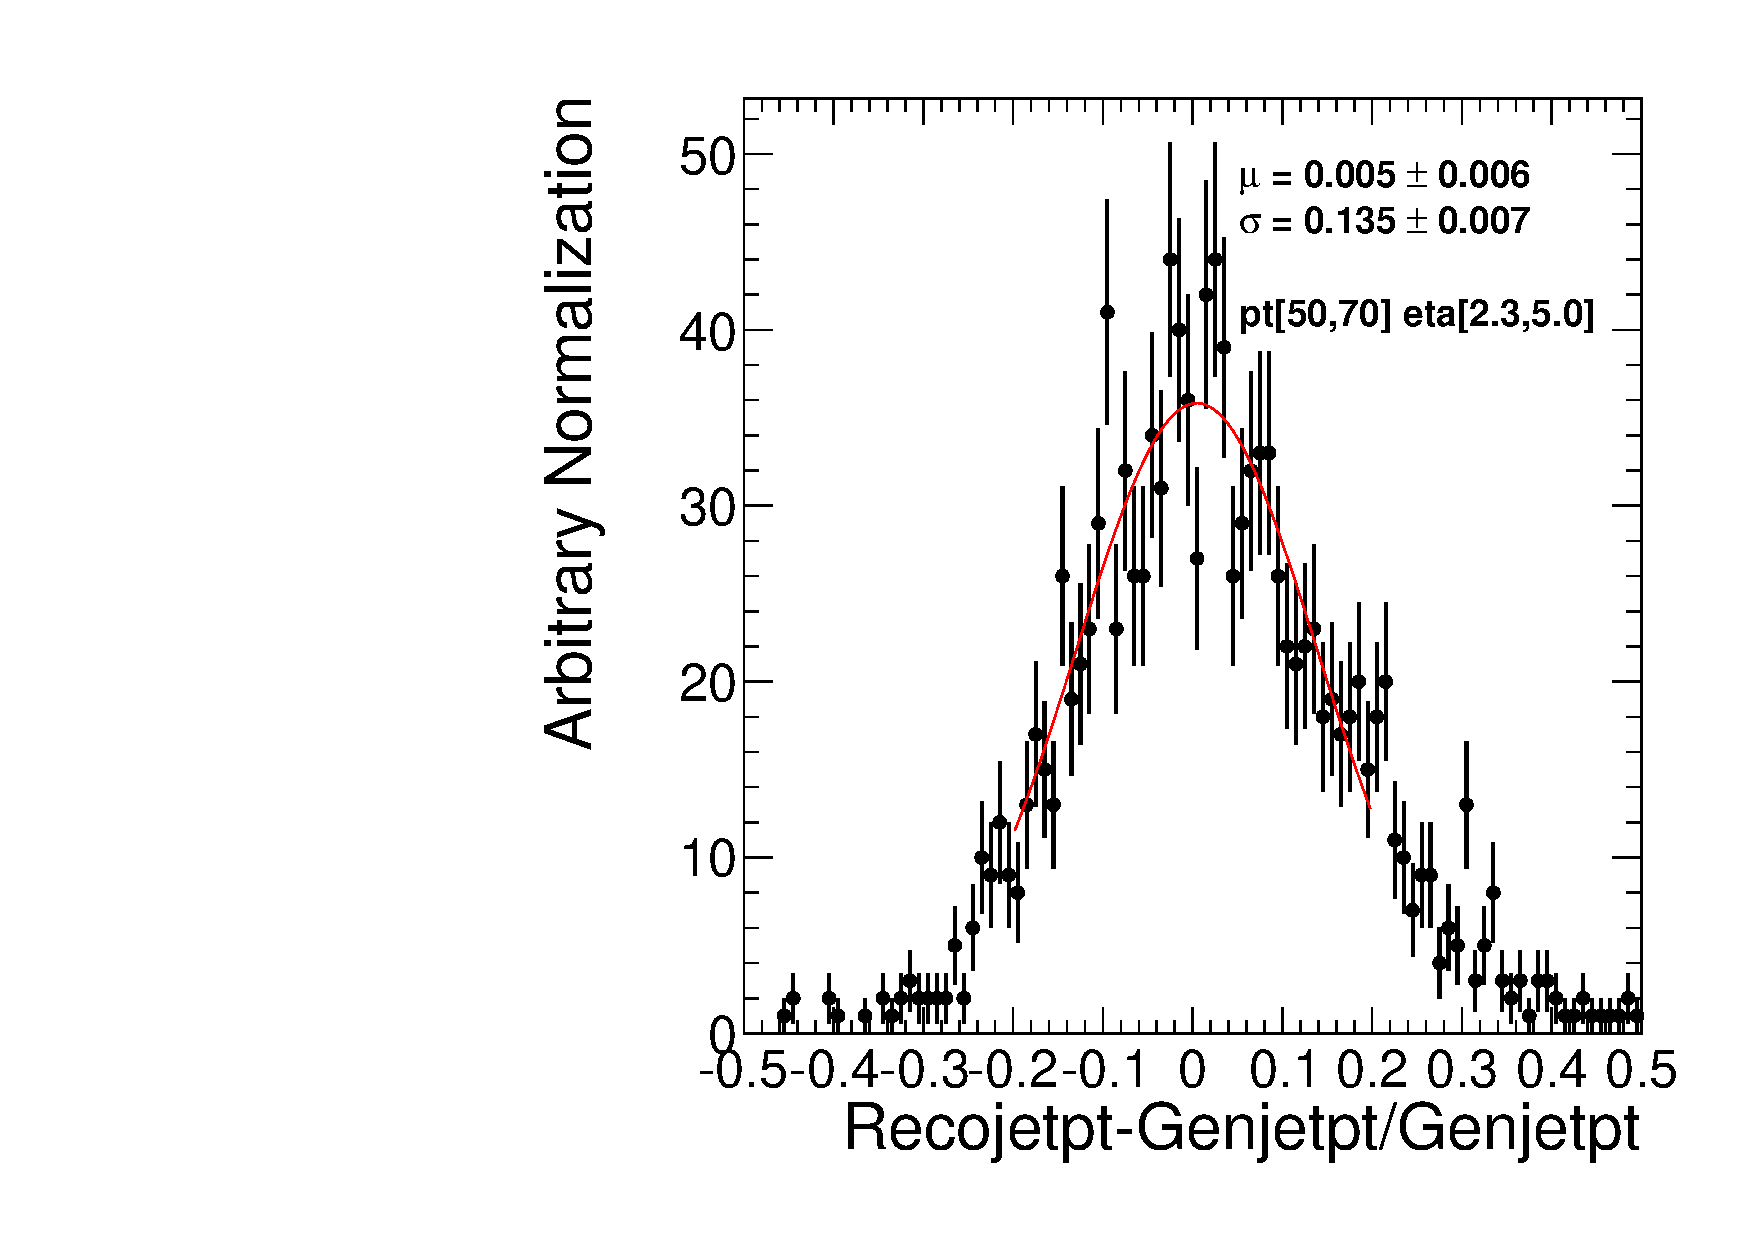
\includegraphics[width=0.45\textwidth]{figs/jer/mu_Recojetpt_Genjetpt_Genjetpt_2_3_5_0_50_70_tagjetresolution_jetresolution.pdf}
\put(-0.80,0.0){(b)} \\  
\unitlength=0.33\linewidth
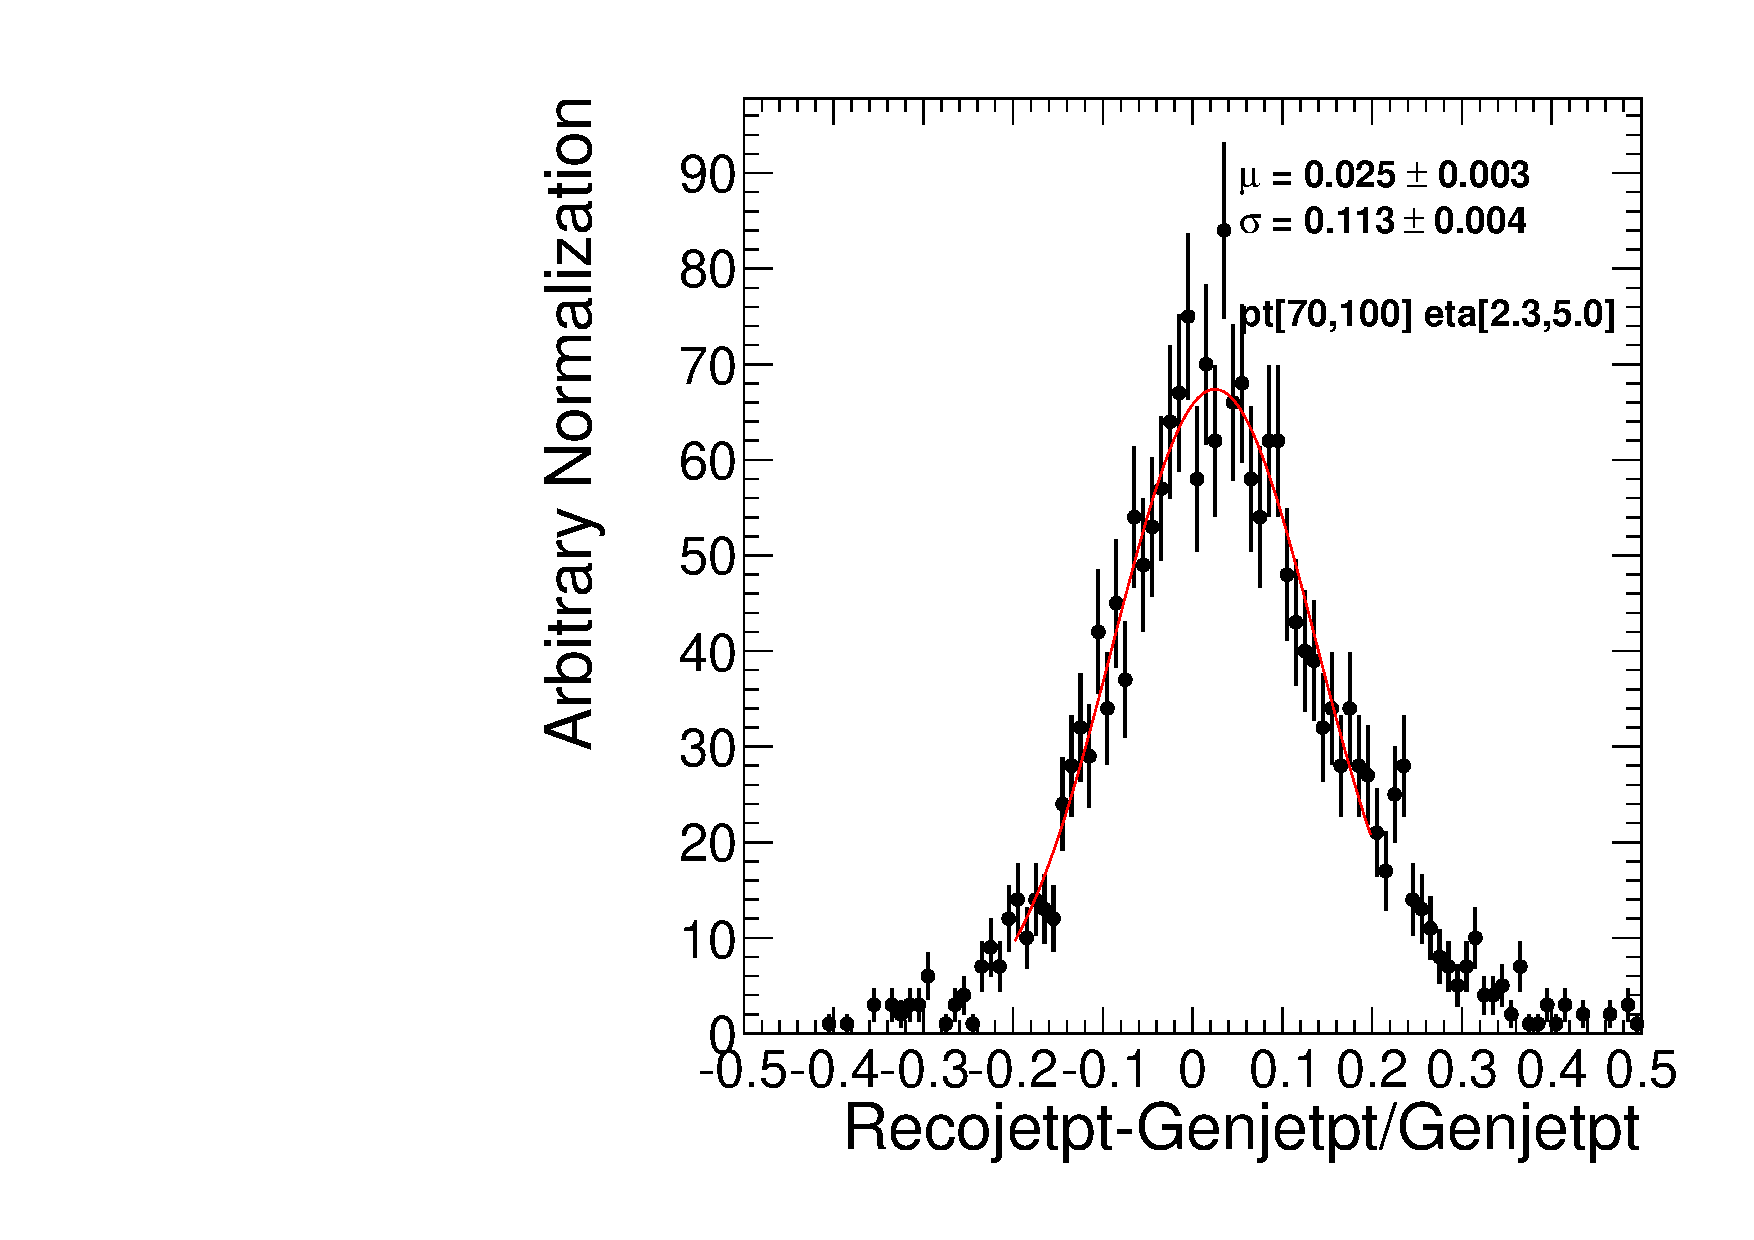
\includegraphics[width=0.45\textwidth]{figs/jer/mu_Recojetpt_Genjetpt_Genjetpt_2_3_5_0_70_100_tagjetresolution_jetresolution.pdf}
\put(-0.80,0.0){(c)}
\unitlength=0.33\linewidth
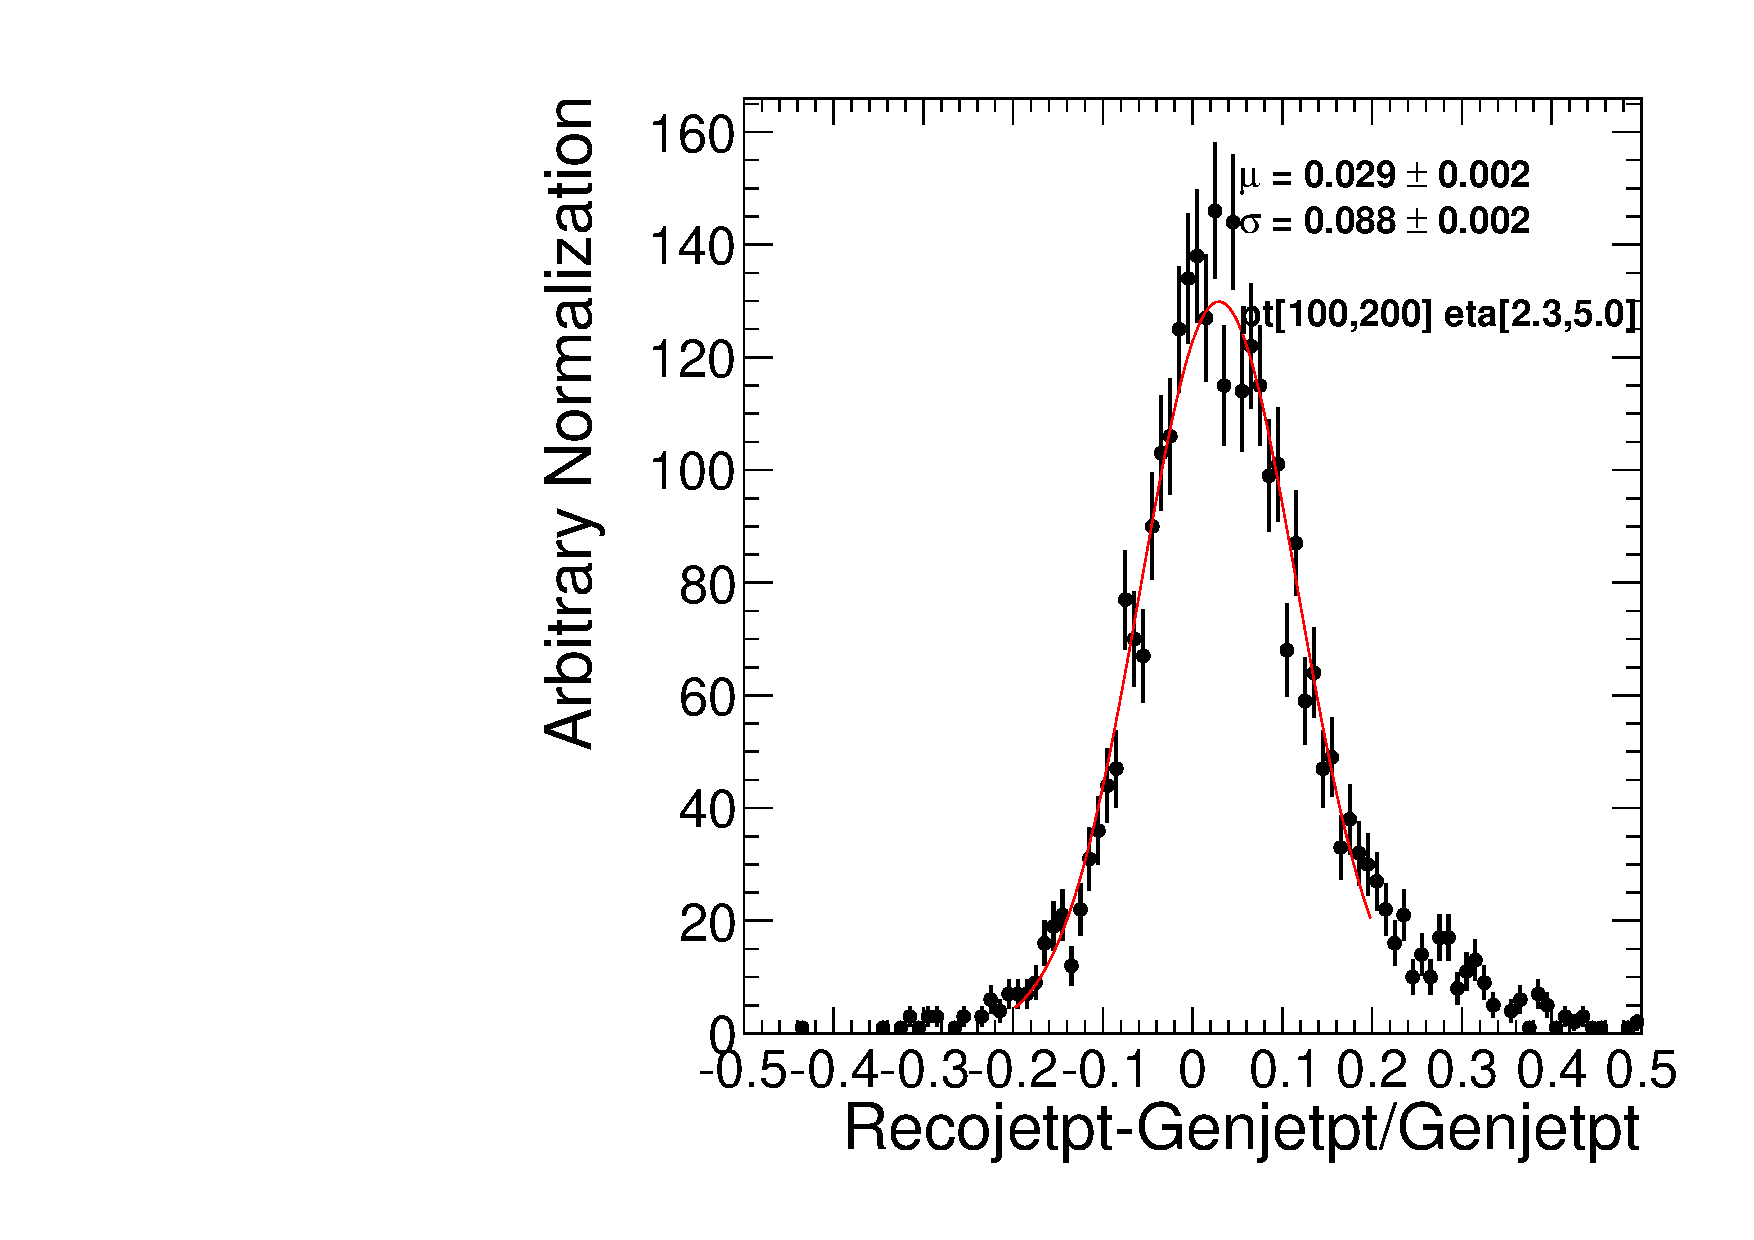
\includegraphics[width=0.45\textwidth]{figs/jer/mu_Recojetpt_Genjetpt_Genjetpt_2_3_5_0_100_200_tagjetresolution_jetresolution.pdf}
\put(-0.80,0.0){(d)}\\ 
\unitlength=0.33\linewidth
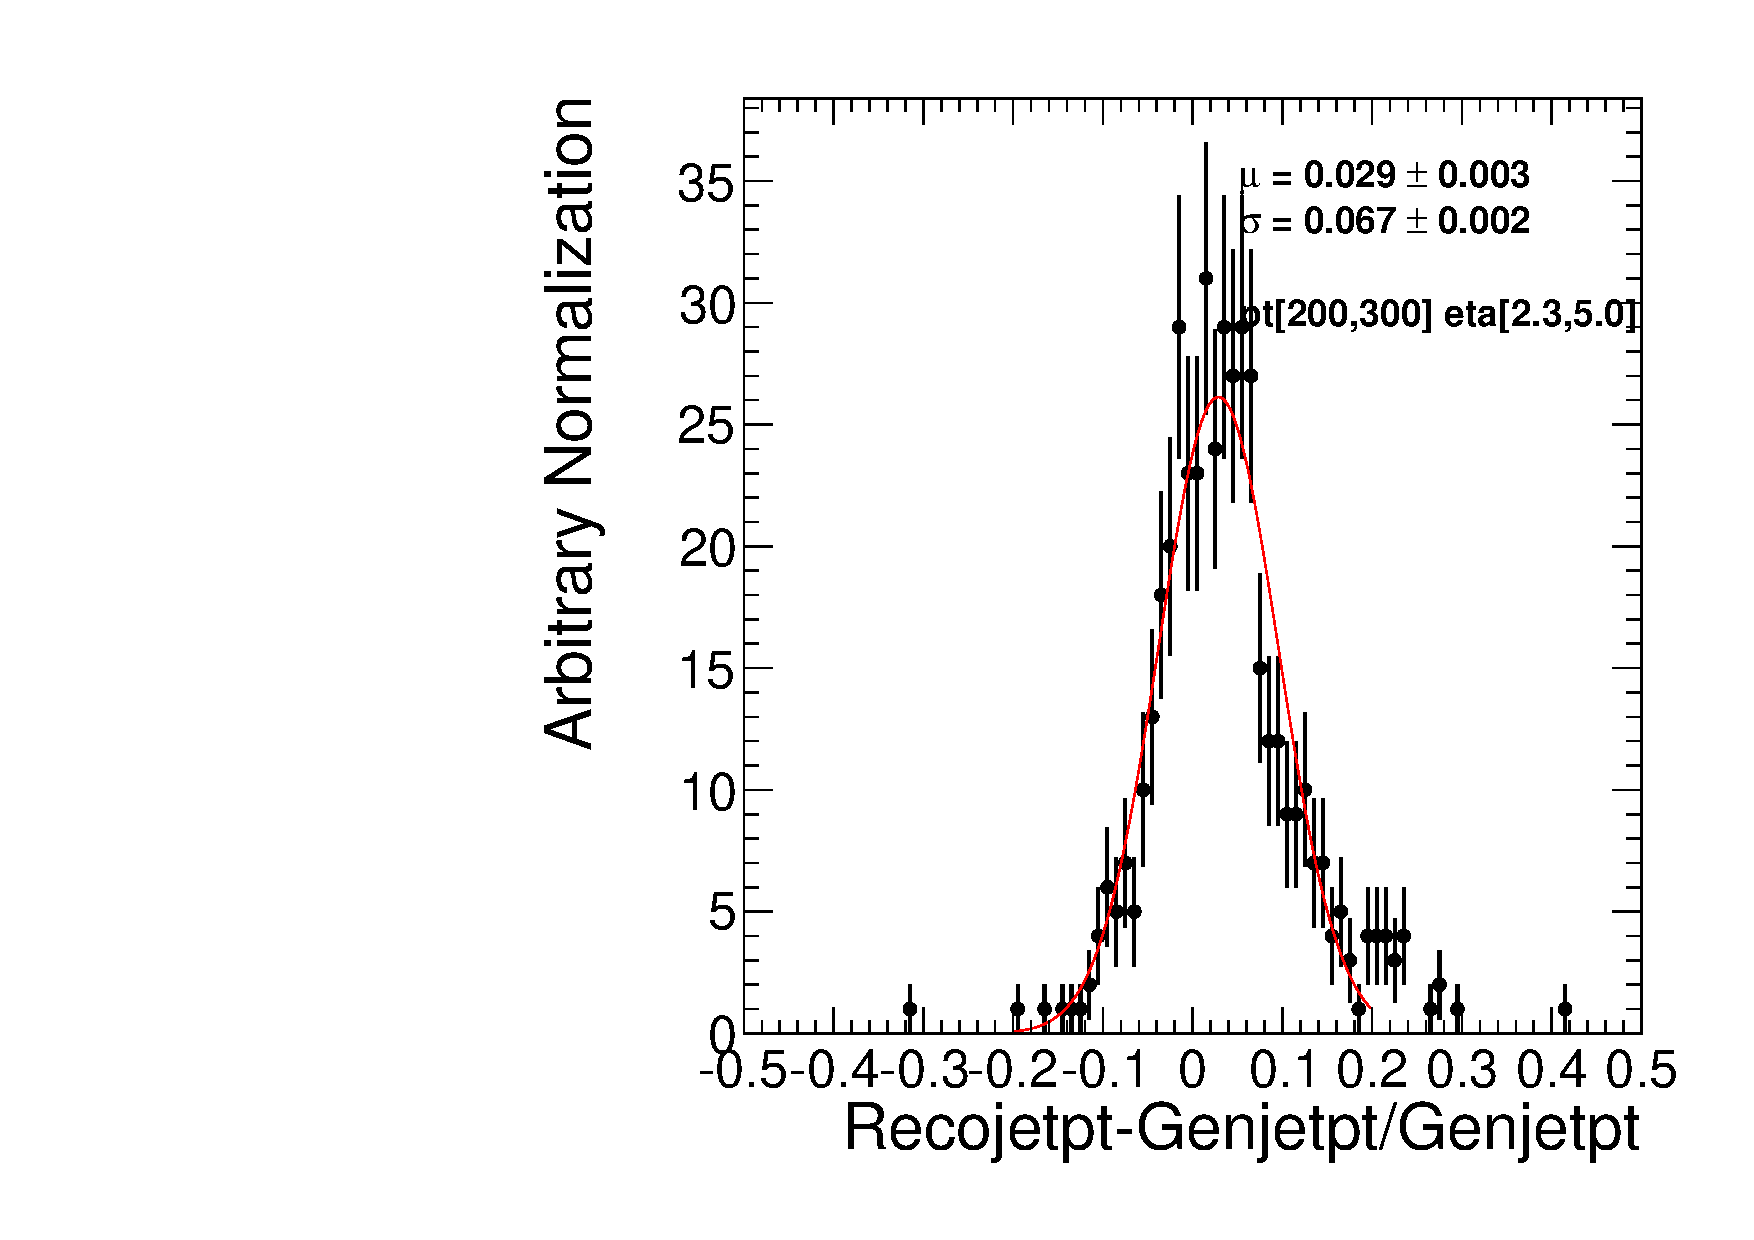
\includegraphics[width=0.45\textwidth]{figs/jer/mu_Recojetpt_Genjetpt_Genjetpt_2_3_5_0_200_300_tagjetresolution_jetresolution.pdf}
\put(-0.80,0.0){(e)} 
\unitlength=0.33\linewidth
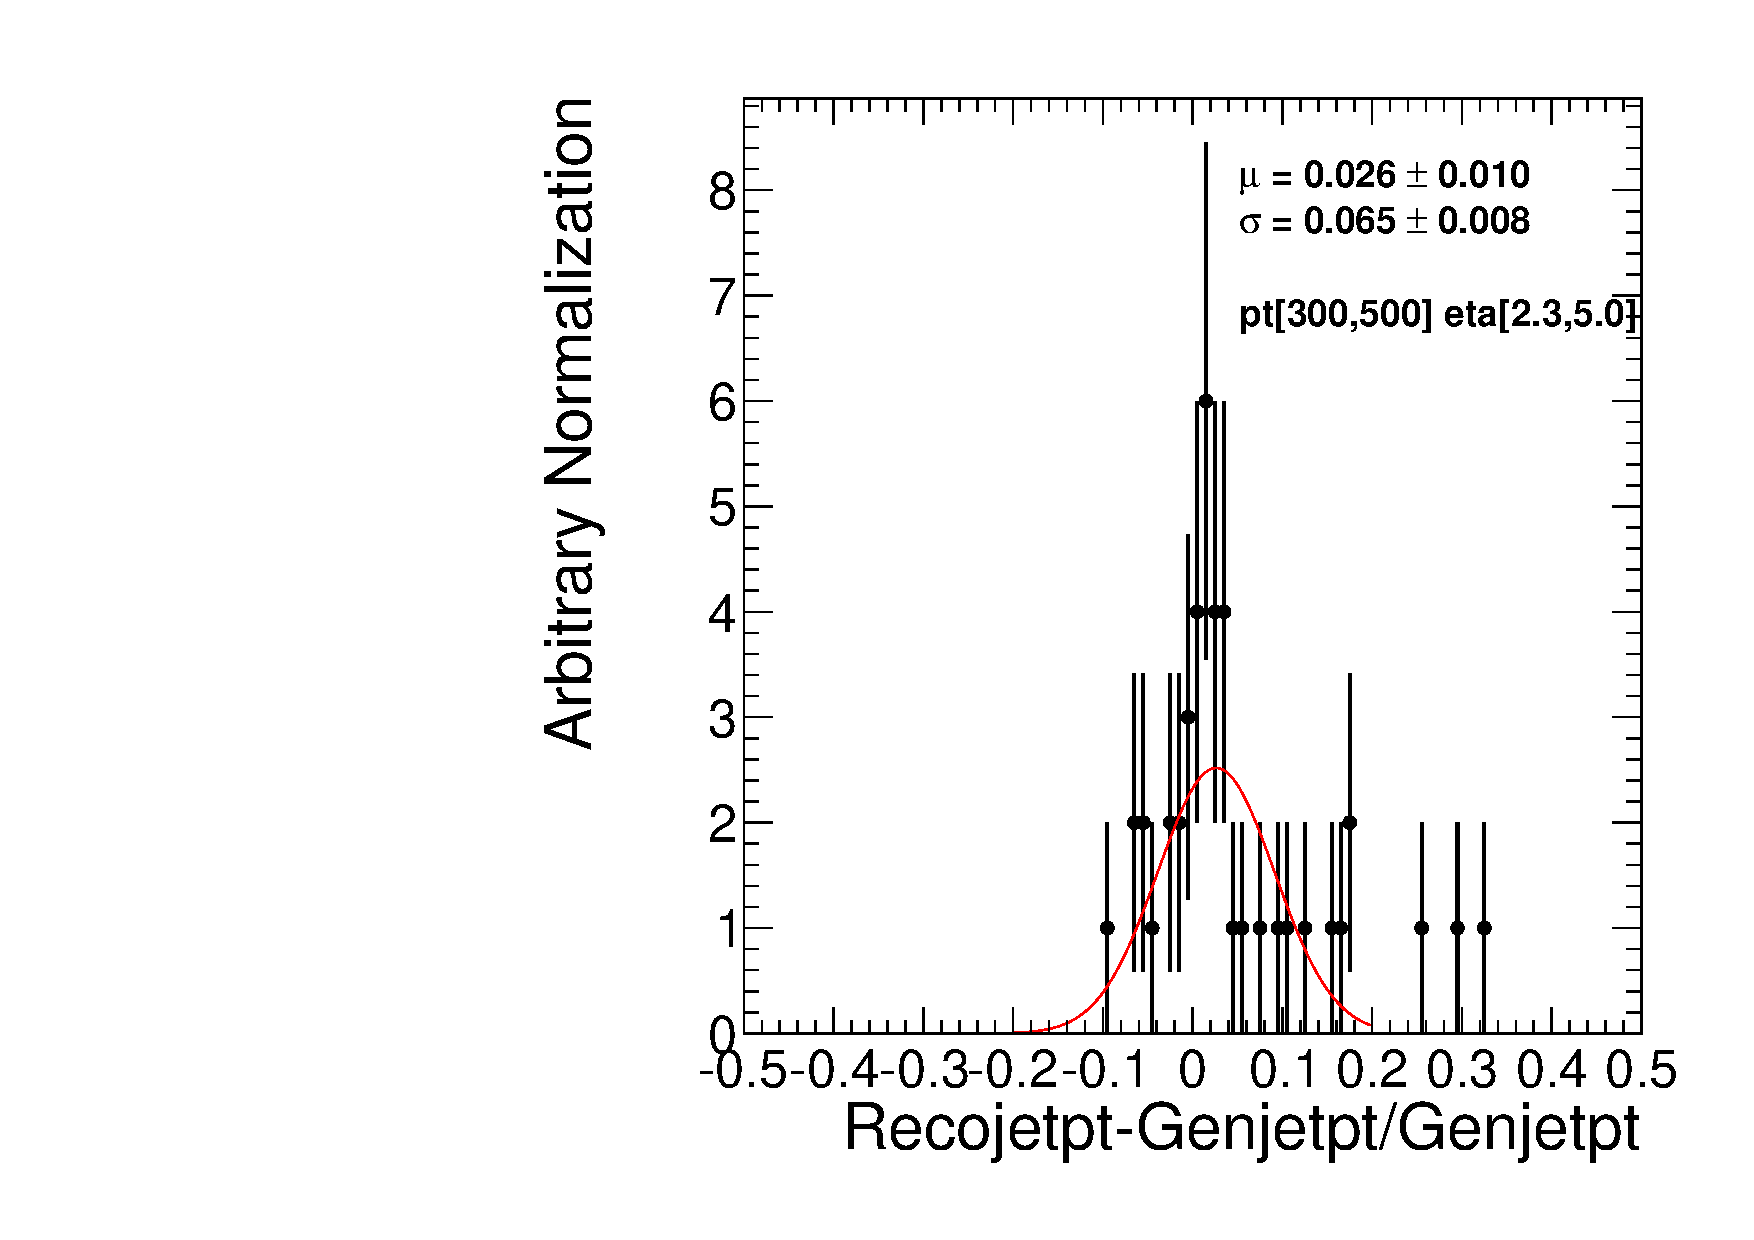
\includegraphics[width=0.45\textwidth]{figs/jer/mu_Recojetpt_Genjetpt_Genjetpt_2_3_5_0_300_500_tagjetresolution_jetresolution.pdf}
\put(-0.80,0.0){(f)} 
\caption{Fit result in jet $\eta$ bin: [2.3, 5.0] for six $p_{T}$[GeV/c] bins: 
         (a) [30, 50], (b) [50, 70], (b) [70, 100], (d) [100, 200], (e) [200, 300], (f) [300, 500].}
\label{fig:jer_eta_5_pt_5}}
\end{figure}

\clearpage
